\begin{longtable}{|p{6.7cm}|p{6.7cm}|}
    \caption{Historia de usuario 1: Iniciar sesión sistema web} \label{tab:historia-1}
    \\
    \hline
    \multicolumn{2}{|c|}{\textbf{Historia de Usuario}}                                                                                                                     \\
    \hline

    \endfirsthead

    \hline
    \endhead

    \hline
    \multicolumn{2}{|c|}{{Continua en la siguiente página}}                                                                                                                \\
    \hline
    \endfoot

    \hline
    \endlastfoot

    \textbf{Número:} 1                                  & \textbf{Usuario:} Usuario administrador                                                                          \\
    \hline
    \multicolumn{2}{|l|}{\textbf{Nombre de la historia:} Iniciar sesión sistema web}                                                                                       \\
    \hline
    \textbf{Prioridad en negocio}  Alta                 & \textbf{Riesgo en desarrollo:} Medio                                                                             \\
    \hline
    \textbf{\textbf{Puntos estimados:}en desarrollo:} 8 & \textbf{Iteración asignada:} 1                                                                                   \\
    \hline
    \multicolumn{2}{|l|}{\textbf{Programador responsable:} José Pazmiño }                                                                                                  \\
    \hline
    \multicolumn{2}{|p{13.4cm}|}{\textbf{Descripción:} Como usuario administrador del sistema web, quiero iniciar sesión en el sistema para acceder a sus funcionalidades} \\
    \hline
    \multicolumn{2}{|c|}{\textbf{Criterios de aceptación}}                                                                                                                 \\
    \hline
    \multicolumn{2}{|p{13.4cm}|}{
    \begin{itemize}[label={},leftmargin=*, nosep]
        \item \textbf{Criterio 1:} Dado que el usuario administrador ingrese su correo y contraseña de forma correcta cuando presione el botón de inicio de sesión, el sistema deberá redirigirlo a la página principal del sistema.
        \item \textbf{Criterio 2:} Dado que el usuario administrador ingrese su correo y contraseña de forma incorrecta cuando presione el botón de inicio de sesión, el sistema deberá mostrar un mensaje de error.
    \end{itemize}
    }                                                                                                                                                                      \\
\end{longtable}


% \begin{figure}[H]
%     \centering
%     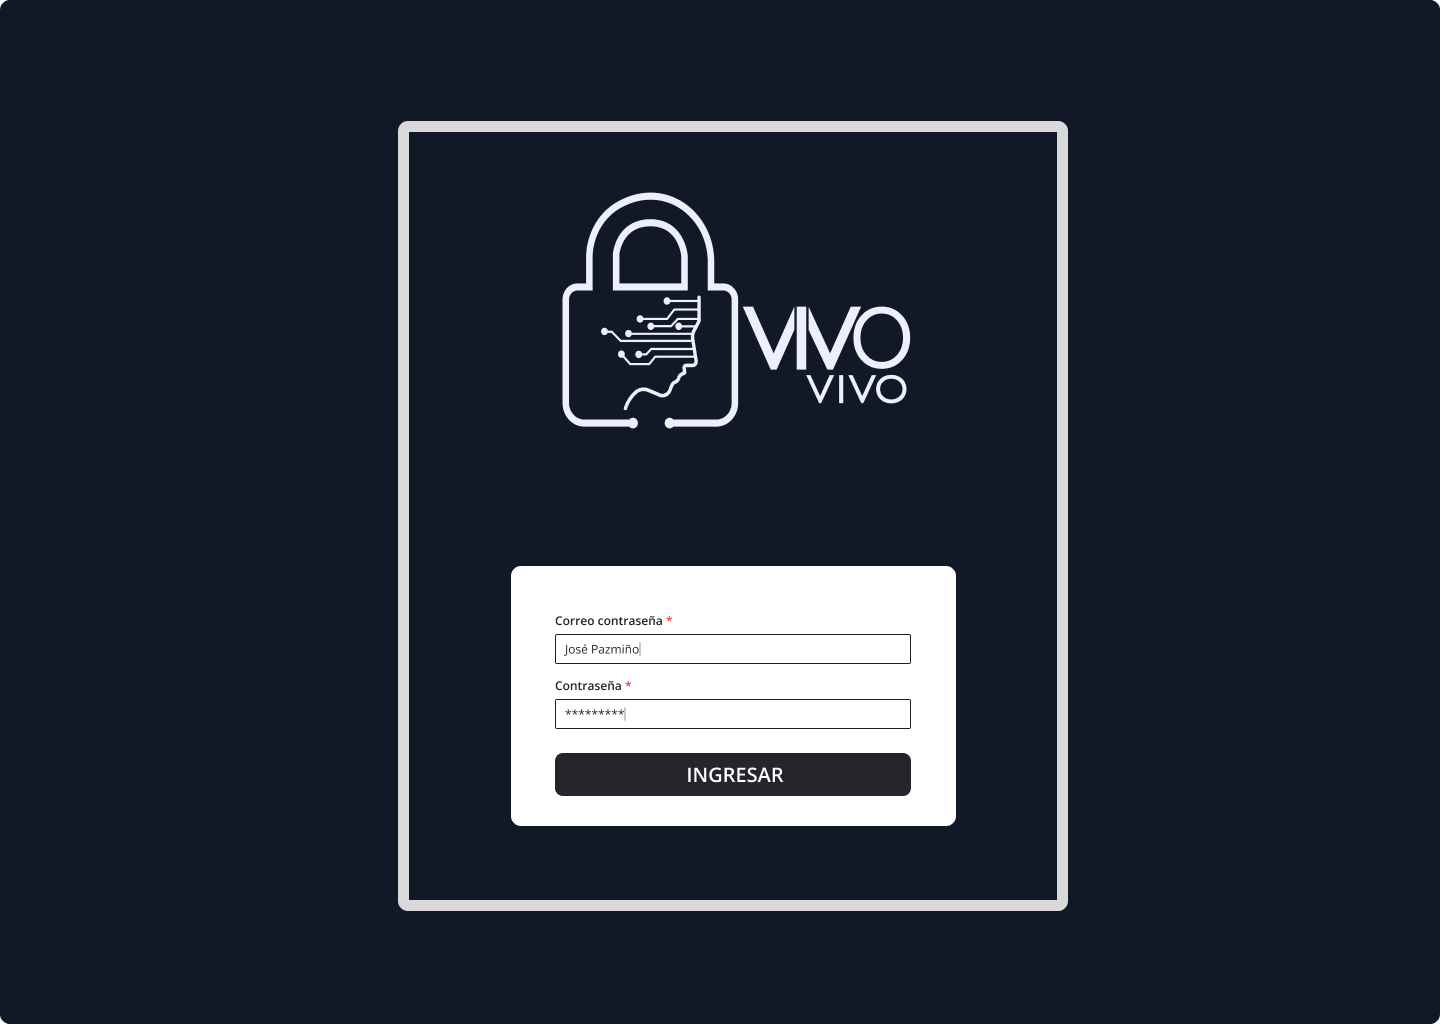
\includegraphics[width=0.6\textwidth]{chapters/III-resultados-y-discusion/resources/images/prototipo-inicio-sesion-web.png}
%     \caption{Prototipo de la interfaz de inicio de sesión web}
%     \label{fig:prototipo-inicio-sesion-web}
% \end{figure}


\begin{longtable}{|p{6.7cm}|p{6.7cm}|}
    \caption{Historia de usuario 2: Cerrar sesión sistema web} \label{tab:historia-2}
    \\
    \hline
    \multicolumn{2}{|c|}{\textbf{Historia de Usuario}}                                                                                                       \\
    \hline

    \endfirsthead

    \hline
    \endhead

    \hline
    \multicolumn{2}{|c|}{{Continua en la siguiente página}}                                                                                                  \\
    \hline
    \endfoot

    \hline
    \endlastfoot

    \textbf{Número:} 2                                  & \textbf{Usuario:} Usuario administrador                                                            \\
    \hline
    \multicolumn{2}{|l|}{\textbf{Nombre de la historia:} Cerrar sesión sistema web}                                                                          \\
    \hline
    \textbf{Prioridad en negocio}  Alta                 & \textbf{Riesgo en desarrollo:} Medio                                                               \\
    \hline
    \textbf{\textbf{Puntos estimados:}en desarrollo:} 2 & \textbf{Iteración asignada:} 1                                                                     \\
    \hline
    \multicolumn{2}{|l|}{\textbf{Programador responsable:} José Pazmiño }                                                                                    \\
    \hline
    \multicolumn{2}{|p{13.4cm}|}{\textbf{Descripción:} Como usuario del sistema web, quiero cerrar sesión en el sistema para finalizar mi sesión de trabajo} \\
    \hline
    \multicolumn{2}{|c|}{\textbf{Criterios de aceptación}}                                                                                                   \\
    \hline
    \multicolumn{2}{|p{13.4cm}|}{
    \begin{itemize}[label={},leftmargin=*, nosep]
        \item \textbf{Criterio 1:} Dado que el usuario administrador presione el botón de cerrar sesión desde cualquier página, el sistema deberá redirigirlo a la página de inicio de sesión.
    \end{itemize}
    }                                                                                                                                                        \\
\end{longtable}


% \begin{figure}[H]
%     \centering
%     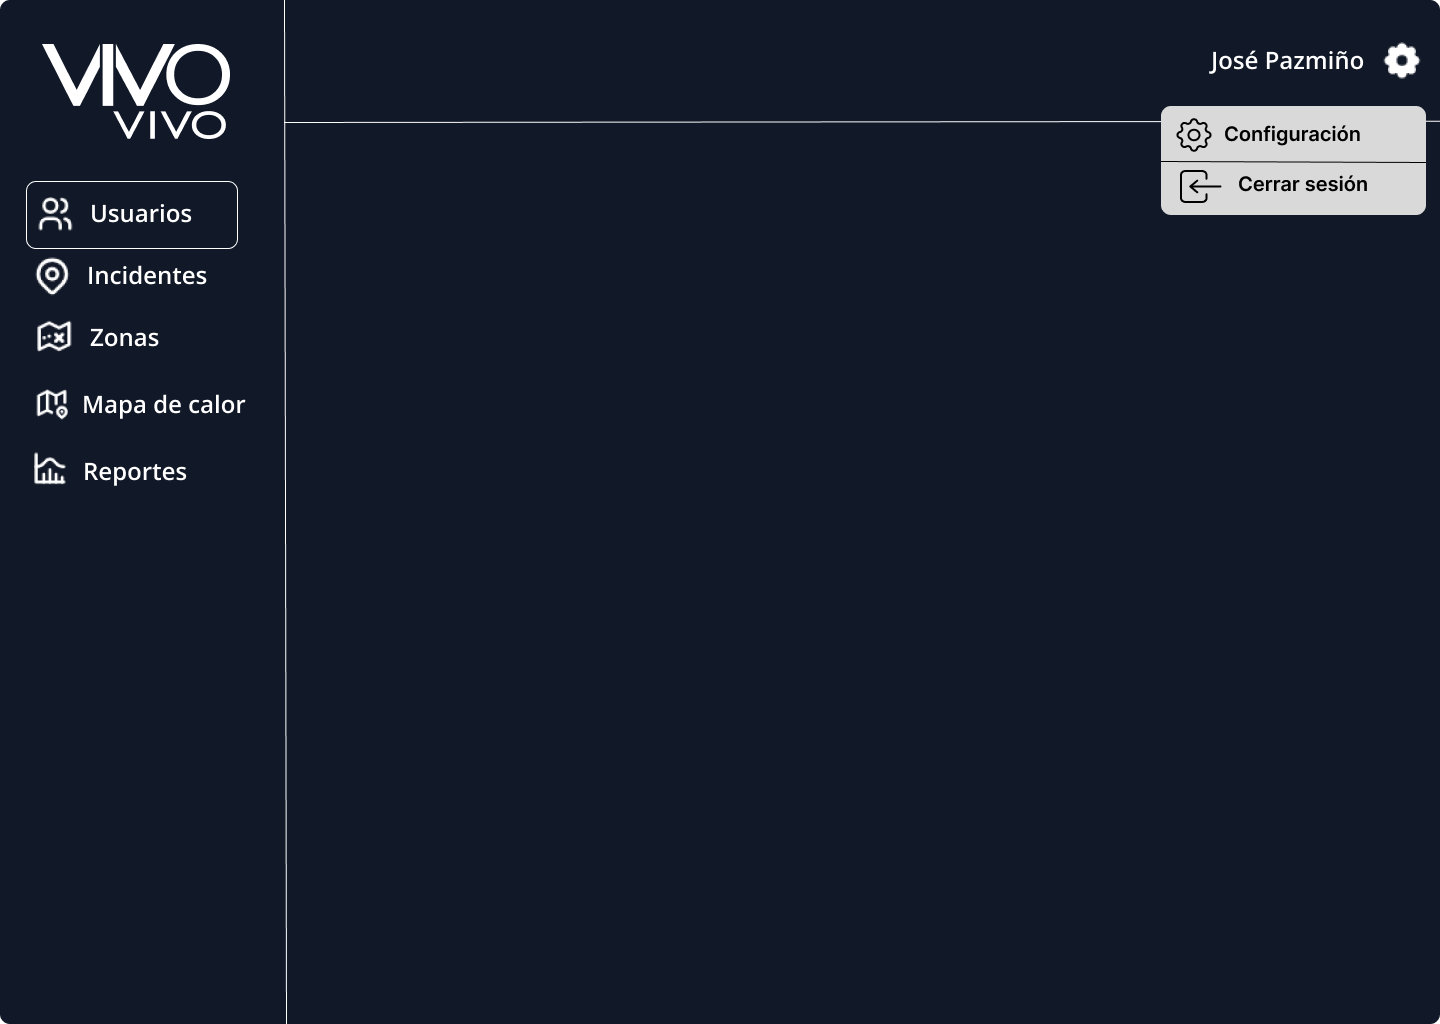
\includegraphics[width=0.6\textwidth]{chapters/III-resultados-y-discusion/resources/images/prototipo-layout-web.png}
%     \caption{Prototipo de la interfaz para cerrar sesión en el sistema web}
%     \label{fig:prototipo-layout-web}
% \end{figure}


\begin{longtable}{|p{6.7cm}|p{6.7cm}|}
    \caption{Historia de usuario 3: Gestionar usuarios} \label{tab:historia-3}
    \\
    \hline
    \multicolumn{2}{|c|}{\textbf{Historia de Usuario}}                                                                                                          \\
    \hline

    \endfirsthead

    \hline
    \endhead

    \hline
    \multicolumn{2}{|c|}{{Continua en la siguiente página}}                                                                                                     \\
    \hline
    \endfoot

    \hline
    \endlastfoot

    \textbf{Número:} 3                                   & \textbf{Usuario:} Usuario administrador                                                              \\
    \hline
    \multicolumn{2}{|l|}{\textbf{Nombre de la historia:} Gestionar usuarios}                                                                                    \\
    \hline
    \textbf{Prioridad en negocio}  Alta                  & \textbf{Riesgo en desarrollo:} Medio                                                                 \\
    \hline
    \textbf{\textbf{Puntos estimados:}en desarrollo:} 18 & \textbf{Iteración asignada:} 1                                                                       \\
    \hline
    \multicolumn{2}{|l|}{\textbf{Programador responsable:} José Pazmiño }                                                                                       \\
    \hline
    \multicolumn{2}{|p{13.4cm}|}{\textbf{Descripción:} Como usuario administrador, quiero administrar los usuarios que se encuentran registrados en el sistema} \\
    \hline
    \multicolumn{2}{|c|}{\textbf{Criterios de aceptación}}                                                                                                      \\
    \hline
    \multicolumn{2}{|p{13.4cm}|}{
    \begin{itemize}[label={},leftmargin=*, nosep]
        \item \textbf{Criterio 1:} El usuario administrador debe poder visualizar, crear, actualizar y deshabilitar y habilitar usuarios en el sistema.
    \end{itemize}
    }                                                                                                                                                           \\
\end{longtable}


% \begin{figure}[H]
%     \centering
%     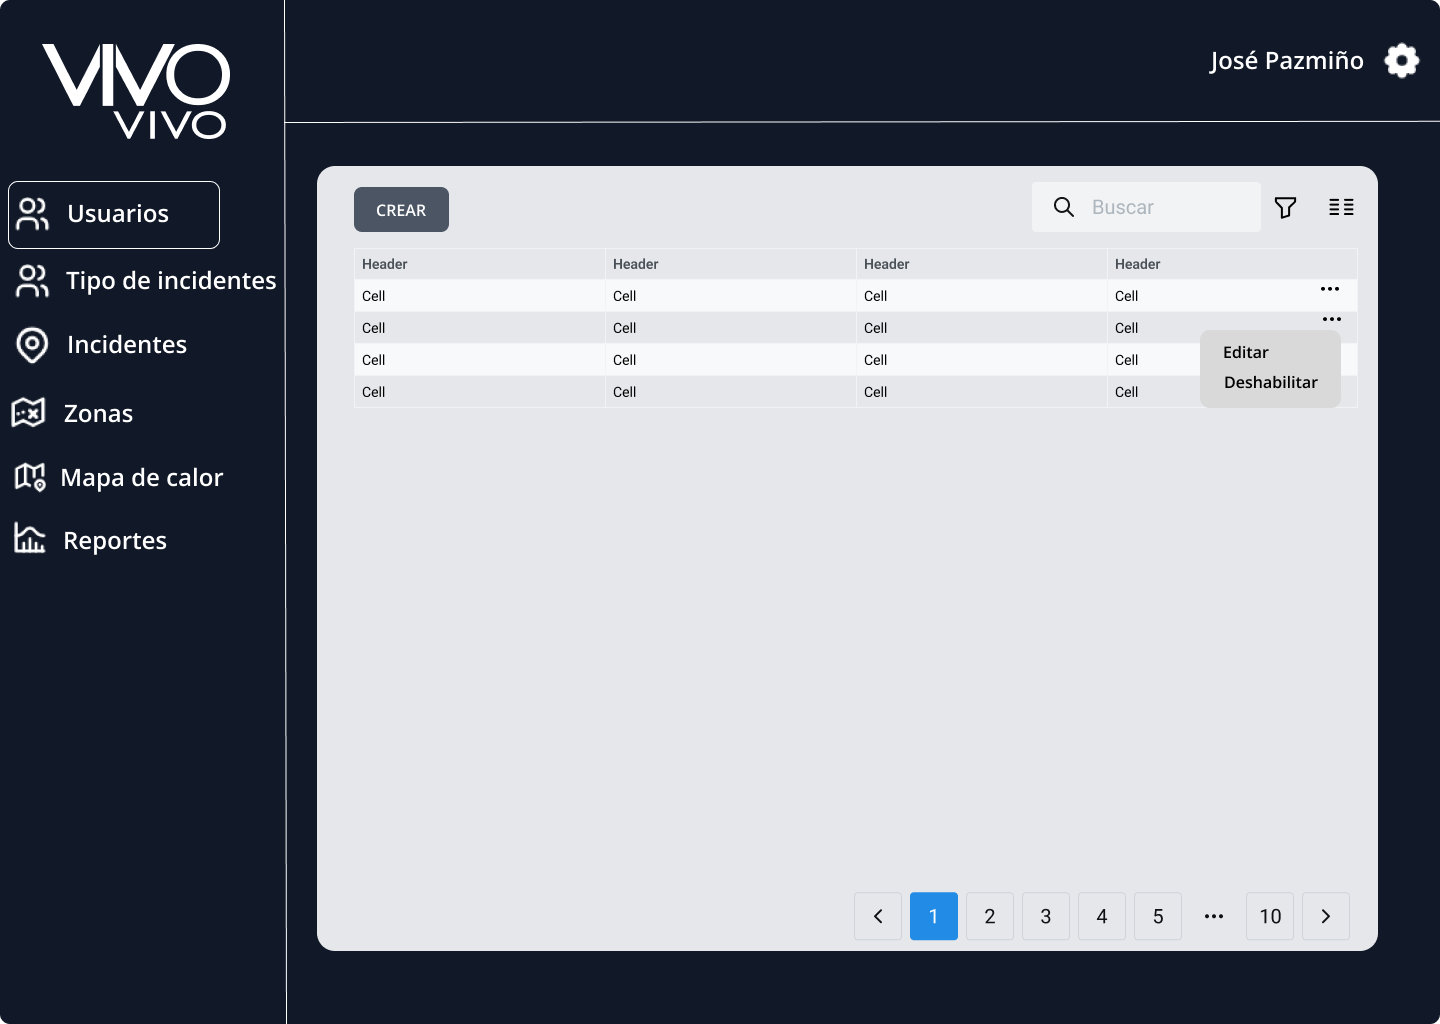
\includegraphics[width=0.6\textwidth]{chapters/III-resultados-y-discusion/resources/images/prototipo-menu-tabla-entradas-web.png}
%     \caption{Prototipo de la interfaz para visualizar los usuarios}
%     \label{fig:prototipo-interfaz-usuario-web-3}
% \end{figure}

% \begin{figure}[H]
%     \centering
%     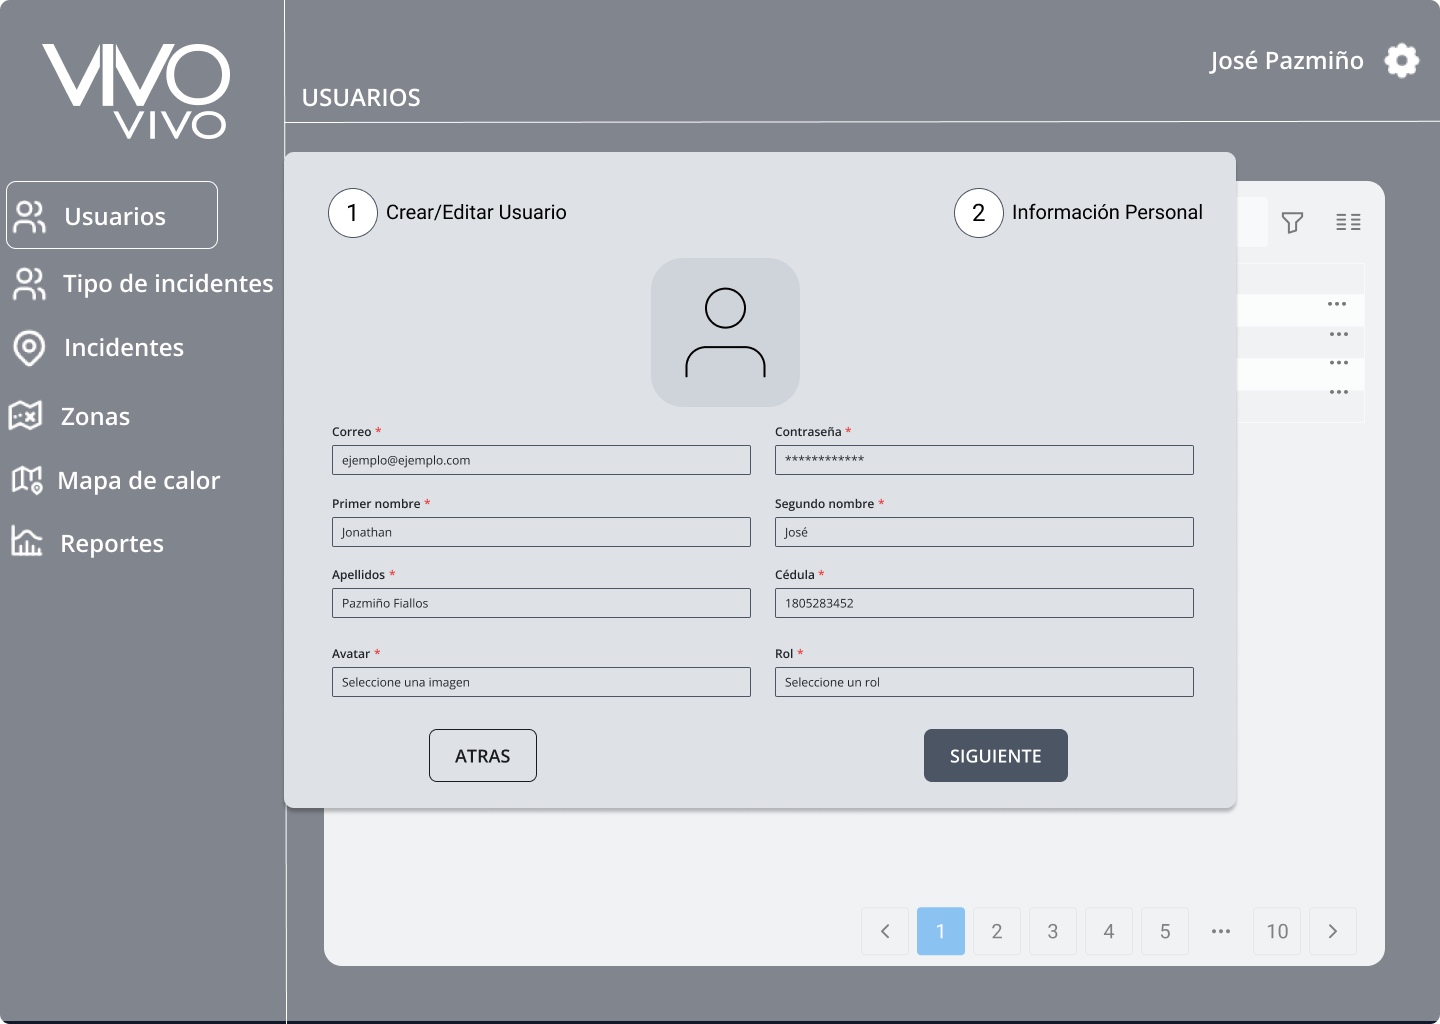
\includegraphics[width=0.6\textwidth]{chapters/III-resultados-y-discusion/resources/images/prototipo-formulario-usuario-web.png}
%     \caption{Prototipo de la interfaz para crear/editar usuario}
%     \label{fig:prototipo-interfaz-usuario-web-4}
% \end{figure}



\begin{longtable}{|p{6.7cm}|p{6.7cm}|}
    \caption{Historia de usuario 4: Gestionar tipos de incidentes} \label{tab:historia-4}
    \\
    \hline
    \multicolumn{2}{|c|}{\textbf{Historia de Usuario}}                                                                                                                     \\
    \hline

    \endfirsthead

    \hline
    \endhead

    \hline
    \multicolumn{2}{|c|}{{Continua en la siguiente página}}                                                                                                                \\
    \hline
    \endfoot

    \hline
    \endlastfoot

    \textbf{Número:} 4                                   & \textbf{Usuario:} Usuario administrador                                                                         \\
    \hline
    \multicolumn{2}{|l|}{\textbf{Nombre de la historia:} Gestionar tipos de incidentes}                                                                                    \\
    \hline
    \textbf{Prioridad en negocio}  Alta                  & \textbf{Riesgo en desarrollo:} Medio                                                                            \\
    \hline
    \textbf{\textbf{Puntos estimados:}en desarrollo:} 13 & \textbf{Iteración asignada:} 1                                                                                  \\
    \hline
    \multicolumn{2}{|l|}{\textbf{Programador responsable:} José Pazmiño }                                                                                                  \\
    \hline
    \multicolumn{2}{|p{13.4cm}|}{\textbf{Descripción:} Como usuario administrador, quiero gestionar los tipos de incidentes para definir las categorías de los incidentes} \\
    \hline
    \multicolumn{2}{|c|}{\textbf{Criterios de aceptación}}                                                                                                                 \\
    \hline
    \multicolumn{2}{|p{13.4cm}|}{
    \begin{itemize}[label={},leftmargin=*, nosep]
        \item \textbf{Criterio 1:} El usuario administrador debe poder visualizar, crear, actualizar y deshabilitar y habilitar tipos de incidentes en el sistema.
    \end{itemize}
    }                                                                                                                                                                      \\
\end{longtable}

% \begin{figure}[H]
%     \centering
%     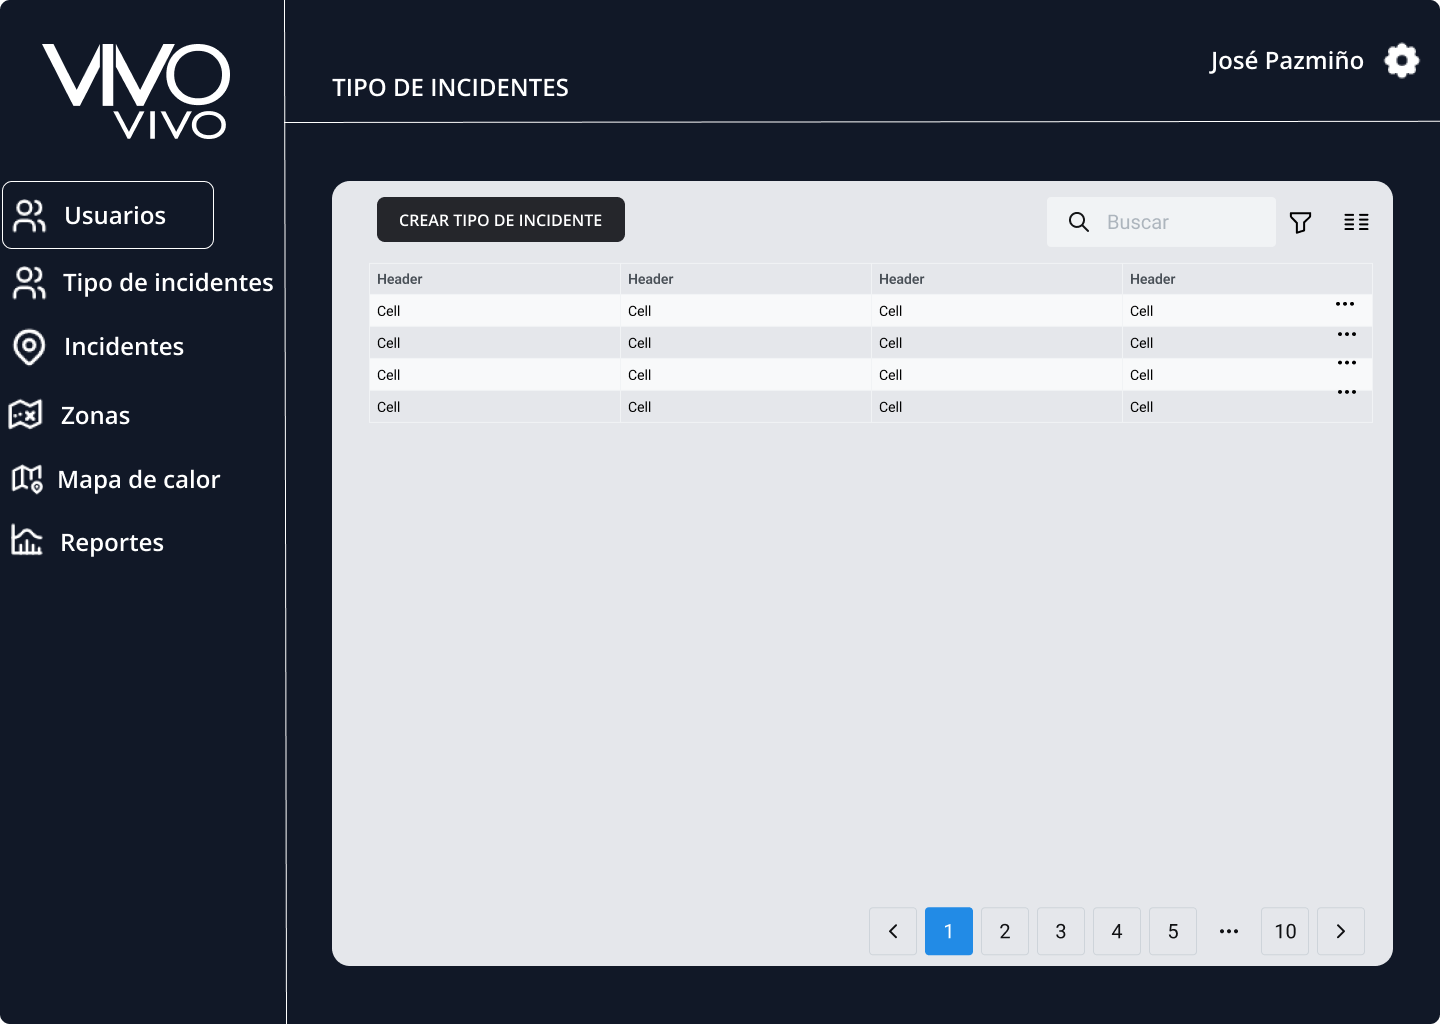
\includegraphics[width=0.6\textwidth]{chapters/III-resultados-y-discusion/resources/images/prototipo-tabla-tipos-incidentes-web.png}
%     \caption{Prototipo de la interfaz para visualizar los tipos de incidentes}
%     \label{fig:prototipo-interfaz-usuario-web-1}
% \end{figure}

% \begin{figure}[H]
%     \centering
%     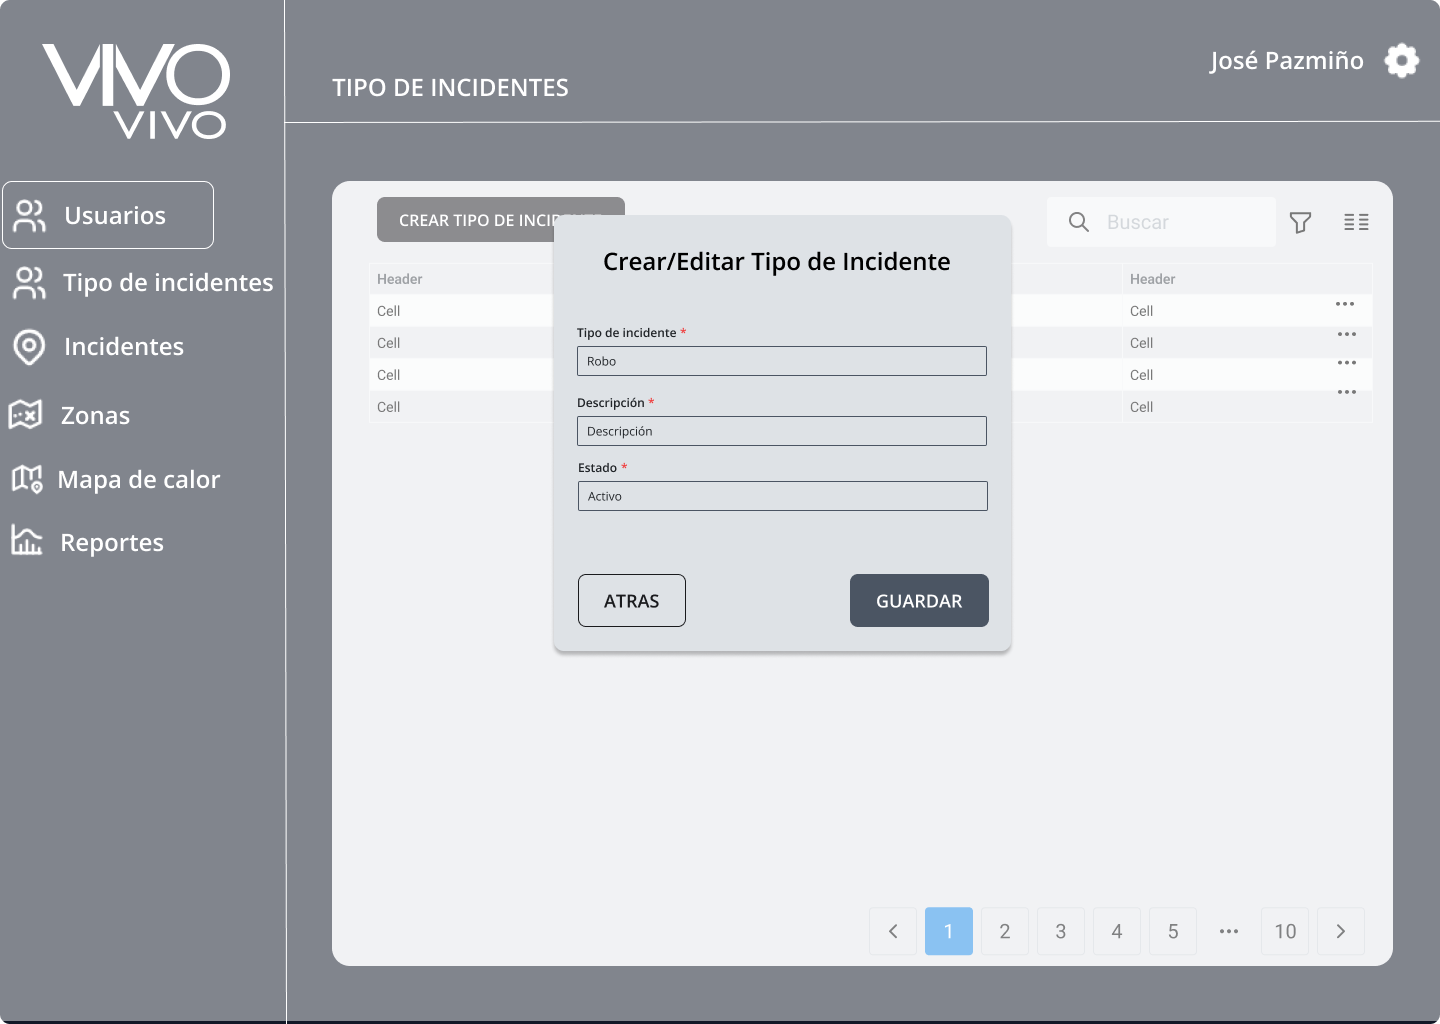
\includegraphics[width=0.6\textwidth]{chapters/III-resultados-y-discusion/resources/images/prototipo-formulario-tipo-incidente-web.png}
%     \caption{Prototipo de la interfaz para crear/editar un tipo de incidente}
%     \label{fig:prototipo-interfaz-usuario-web-2}
% \end{figure}


\begin{longtable}{|p{6.7cm}|p{6.7cm}|}
    \caption{Historia de usuario 5: Gestionar zonas de vigilancia} \label{tab:historia-5}
    \\
    \hline
    \multicolumn{2}{|c|}{\textbf{Historia de Usuario}}                                                                                                           \\
    \hline

    \endfirsthead

    \hline
    \endhead

    \hline
    \multicolumn{2}{|c|}{{Continua en la siguiente página}}                                                                                                      \\
    \hline
    \endfoot

    \hline
    \endlastfoot

    \textbf{Número:} 5                                   & \textbf{Usuario:} Usuario administrador                                                               \\
    \hline
    \multicolumn{2}{|l|}{\textbf{Nombre de la historia:} Gestionar zonas de vigilancia}                                                                          \\
    \hline
    \textbf{Prioridad en negocio}  Alta                  & \textbf{Riesgo en desarrollo:} Medio                                                                  \\
    \hline
    \textbf{\textbf{Puntos estimados:}en desarrollo:} 21 & \textbf{Iteración asignada:} 2                                                                        \\
    \hline
    \multicolumn{2}{|l|}{\textbf{Programador responsable:} José Pazmiño }                                                                                        \\
    \hline
    \multicolumn{2}{|p{13.4cm}|}{\textbf{Descripción:} Como usuario administrador, quiero gestionar las zonas de vigilancia para definir las áreas de monitoreo} \\
    \hline
    \multicolumn{2}{|c|}{\textbf{Criterios de aceptación}}                                                                                                       \\
    \hline
    \multicolumn{2}{|p{13.4cm}|}{
    \begin{itemize}[label={},leftmargin=*, nosep]
        \item \textbf{Criterio 1:} El usuario administrador debe poder visualizar, crear, actualizar y deshabilitar y habilitar zonas de vigilancia en el sistema.
    \end{itemize}
    }                                                                                                                                                            \\
\end{longtable}

% \begin{figure}[H]
%     \centering
%     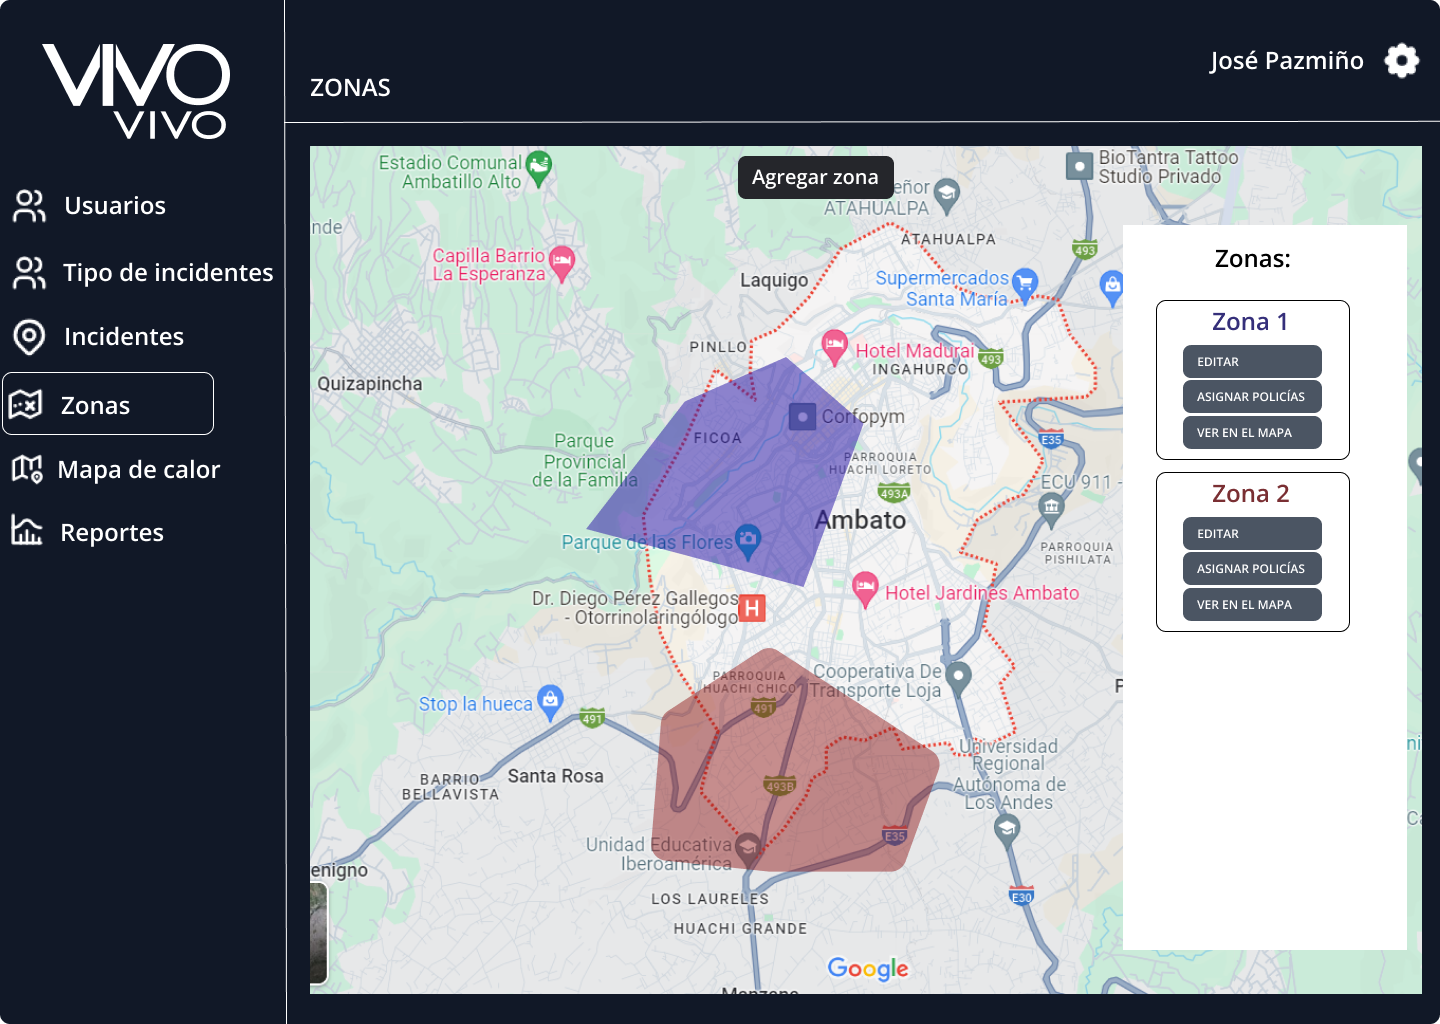
\includegraphics[width=0.6\textwidth]{chapters/III-resultados-y-discusion/resources/images/prototipo-mapa-zonas-de-vigilancia-web.png}
%     \caption{Prototipo de la interfaz para visualizar las zonas de vigilancia}
%     \label{fig:prototipo-interfaz-usuario-web-5}
% \end{figure}

% \begin{figure}[H]
%     \centering
%     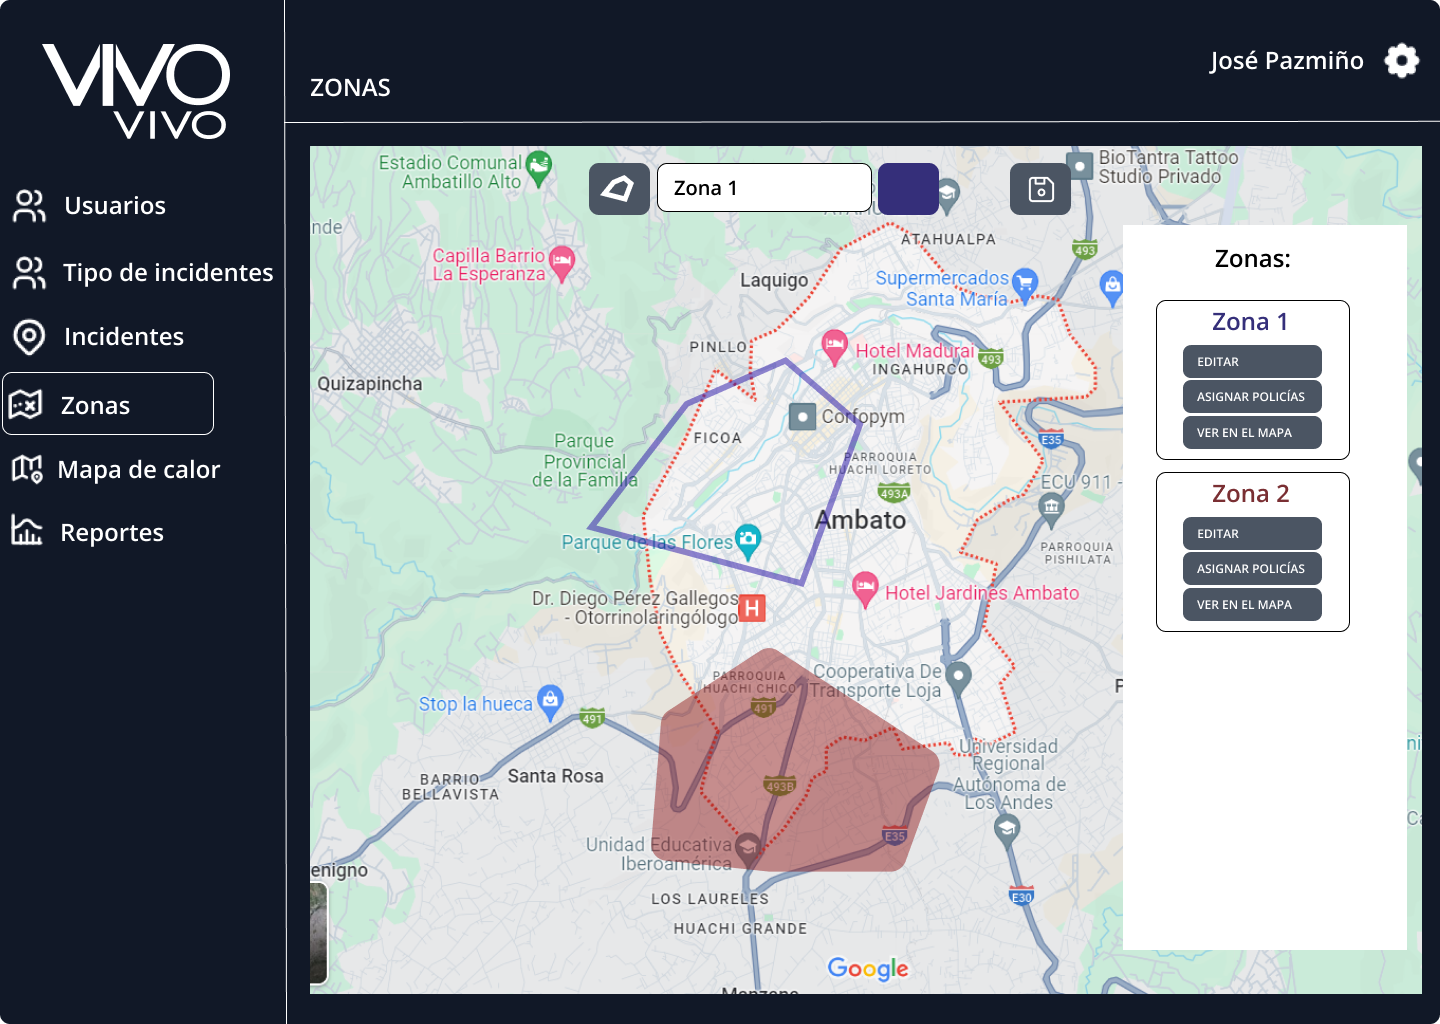
\includegraphics[width=0.6\textwidth]{chapters/III-resultados-y-discusion/resources/images/prototipo-formulario-zona-vigilancia-web.png}
%     \caption{Prototipo de la interfaz para crear/editar una zona de vigilancia}
%     \label{fig:prototipo-interfaz-usuario-web-6}
% \end{figure}



\begin{longtable}{|p{6.7cm}|p{6.7cm}|}
    \caption{Historia de usuario 6: Asignar policías a las zonas de vigilancia} \label{tab:historia-6}
    \\
    \hline
    \multicolumn{2}{|c|}{\textbf{Historia de Usuario}}                                                                                                           \\
    \hline

    \endfirsthead

    \hline
    \endhead

    \hline
    \multicolumn{2}{|c|}{{Continua en la siguiente página}}                                                                                                      \\
    \hline
    \endfoot

    \hline
    \endlastfoot

    \textbf{Número:} 6                                   & \textbf{Usuario:} Usuario administrador                                                               \\
    \hline
    \multicolumn{2}{|l|}{\textbf{Nombre de la historia:} Asignar policías a las zonas de vigilancia}                                                             \\
    \hline
    \textbf{Prioridad en negocio}  Alta                  & \textbf{Riesgo en desarrollo:} Medio                                                                  \\
    \hline
    \textbf{\textbf{Puntos estimados:}en desarrollo:} 13 & \textbf{Iteración asignada:} 2                                                                        \\
    \hline
    \multicolumn{2}{|l|}{\textbf{Programador responsable:} José Pazmiño }                                                                                        \\
    \hline
    \multicolumn{2}{|p{13.4cm}|}{\textbf{Descripción:} Como usuario administrador, quiero asignar y desasignar miembros de la policía a las zonas de vigilancia} \\
    \hline
    \multicolumn{2}{|c|}{\textbf{Criterios de aceptación}}                                                                                                       \\
    \hline
    \multicolumn{2}{|p{13.4cm}|}{
    \begin{itemize}[label={},leftmargin=*, nosep]
        \item \textbf{Criterio 1:} El usuario administrador debe poder visualizar, asignar y desasignar miembros de la policía a las zonas de vigilancia en el sistema.
    \end{itemize}
    }                                                                                                                                                            \\
\end{longtable}


% \begin{figure}[H]
%     \centering
%     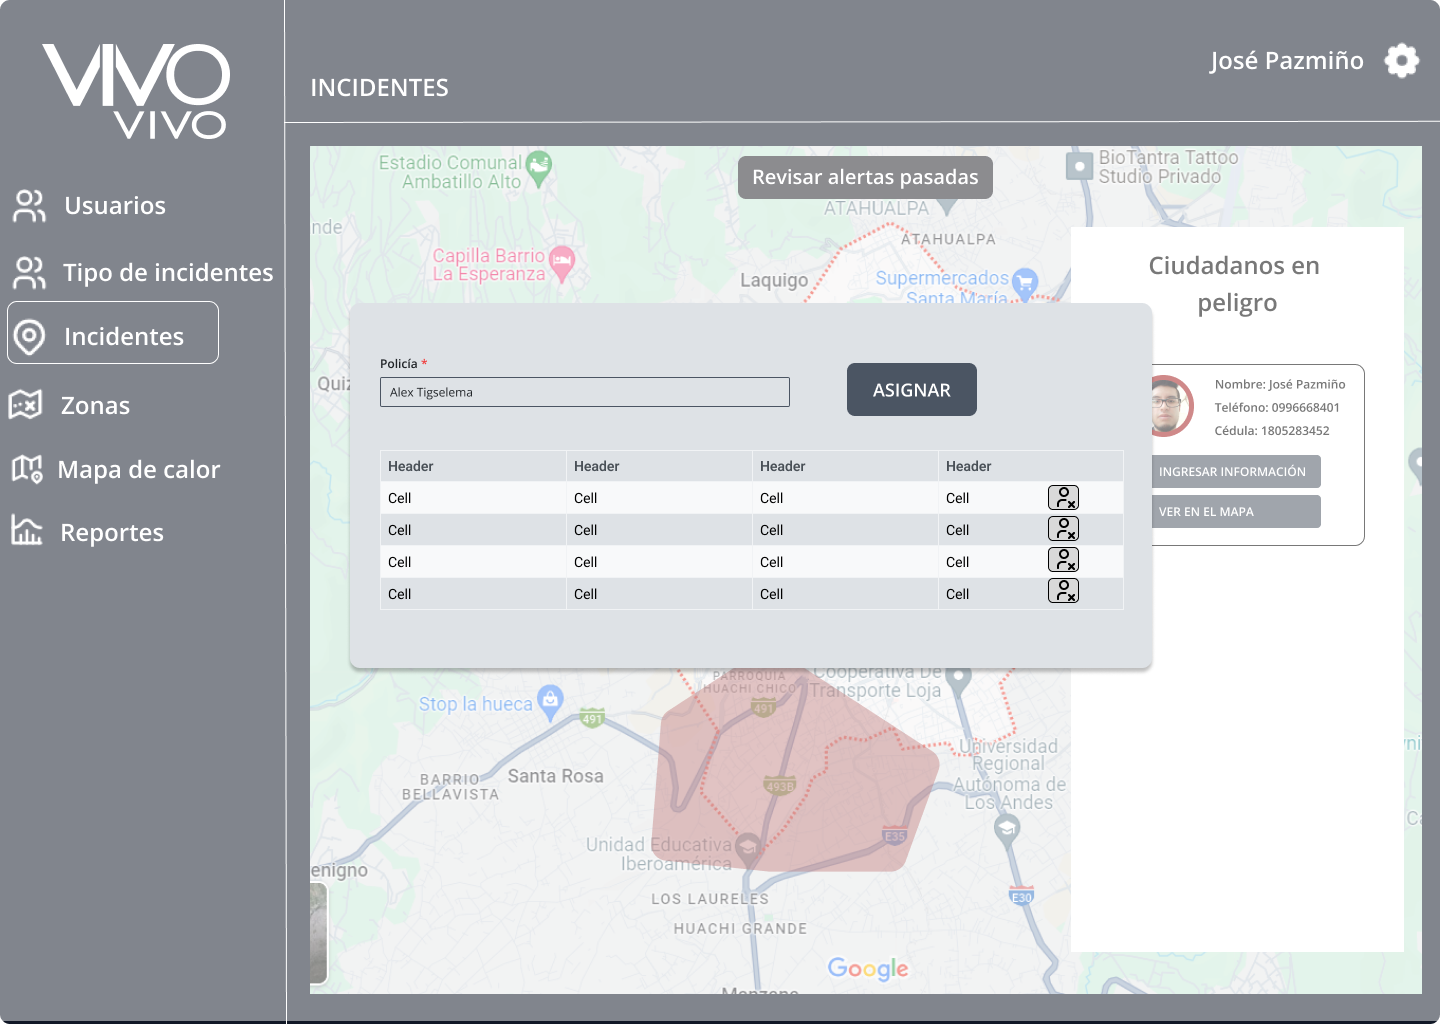
\includegraphics[width=0.6\textwidth]{chapters/III-resultados-y-discusion/resources/images/prototipo-asignar-policias-zona-vigilancia.png}
%     \caption{Prototipo de la interfaz para asignar/desasignar policías a la zona de vigilancia}
%     \label{fig:prototipo-interfaz-usuario-web-7}
% \end{figure}


\begin{longtable}{|p{6.7cm}|p{6.7cm}|}
    \caption{Historia de usuario 7: Gestionar alertas de incidentes} \label{tab:historia-7}
    \\
    \hline
    \multicolumn{2}{|c|}{\textbf{Historia de Usuario}}                                                                                                                                                           \\
    \hline

    \endfirsthead

    \hline
    \endhead

    \hline
    \multicolumn{2}{|c|}{{Continua en la siguiente página}}                                                                                                                                                      \\
    \hline
    \endfoot

    \hline
    \endlastfoot

    \textbf{Número:} 7                                   & \textbf{Usuario:} Usuario administrador                                                                                                               \\
    \hline
    \multicolumn{2}{|l|}{\textbf{Nombre de la historia:} Gestionar alertas de incidentes}                                                                                                                        \\
    \hline
    \textbf{Prioridad en negocio}  Alta                  & \textbf{Riesgo en desarrollo:} Medio                                                                                                                  \\
    \hline
    \textbf{\textbf{Puntos estimados:}en desarrollo:} 23 & \textbf{Iteración asignada:} 2                                                                                                                        \\
    \hline
    \multicolumn{2}{|l|}{\textbf{Programador responsable:} José Pazmiño }                                                                                                                                        \\
    \hline
    \multicolumn{2}{|p{13.4cm}|}{\textbf{Descripción:} Como usuario administrador, quiero visualizar mediante un mapa las alertas de emergencia enviadas por los ciudadanos así como su posición en tiempo real} \\
    \hline
    \multicolumn{2}{|c|}{\textbf{Criterios de aceptación}}                                                                                                                                                       \\
    \hline
    \multicolumn{2}{|p{13.4cm}|}{
    \begin{itemize}[label={},leftmargin=*, nosep]
        \item \textbf{Criterio 1:} El usuario administrador debe poder visualizar mediante un mapa las alertas de emergencia enviadas por los ciudadanos así como su posición en tiempo real.
    \end{itemize}
    }                                                                                                                                                                                                            \\
\end{longtable}


% \begin{figure}[H]
%     \centering
%     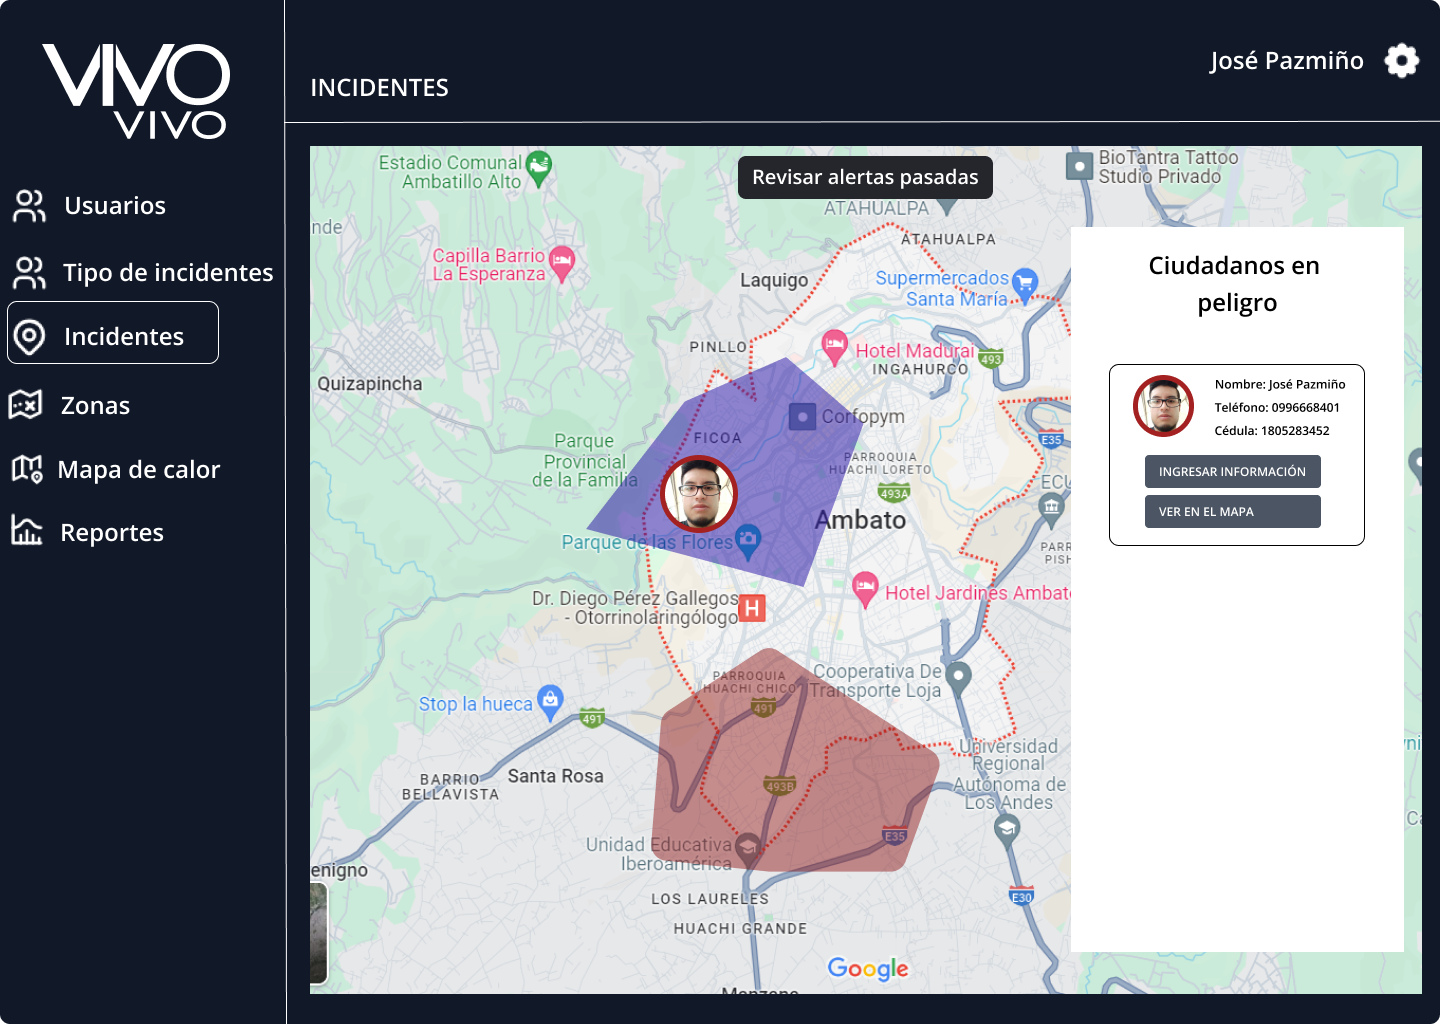
\includegraphics[width=0.6\textwidth]{chapters/III-resultados-y-discusion/resources/images/prototipo-mapa-incidentes-web.png}
%     \caption{Prototipo de la interfaz para visualizar las alertas de incidentes}
%     \label{fig:prototipo-interfaz-usuario-web-8}
% \end{figure}


\begin{longtable}{|p{6.7cm}|p{6.7cm}|}
    \caption{Historia de usuario 8: Visualizar mapa de calor} \label{tab:historia-8}
    \\
    \hline
    \multicolumn{2}{|c|}{\textbf{Historia de Usuario}}                                                                                                                                       \\
    \hline

    \endfirsthead

    \hline
    \endhead

    \hline
    \multicolumn{2}{|c|}{{Continua en la siguiente página}}                                                                                                                                  \\
    \hline
    \endfoot

    \hline
    \endlastfoot

    \textbf{Número:} 8                                   & \textbf{Usuario:} Usuario administrador                                                                                           \\
    \hline
    \multicolumn{2}{|l|}{\textbf{Nombre de la historia:} Visualizar mapa de calor}                                                                                                           \\
    \hline
    \textbf{Prioridad en negocio}  Alta                  & \textbf{Riesgo en desarrollo:} Medio                                                                                              \\
    \hline
    \textbf{\textbf{Puntos estimados:}en desarrollo:} 11 & \textbf{Iteración asignada:} 2                                                                                                    \\
    \hline
    \multicolumn{2}{|l|}{\textbf{Programador responsable:} José Pazmiño }                                                                                                                    \\
    \hline
    \multicolumn{2}{|p{13.4cm}|}{\textbf{Descripción:} Como usuario administrador, quiero visualizar mediante un mapa de calor los incidentes delictivos suscitados en las diferentes zonas} \\
    \hline
    \multicolumn{2}{|c|}{\textbf{Criterios de aceptación}}                                                                                                                                   \\
    \hline
    \multicolumn{2}{|p{13.4cm}|}{
    \begin{itemize}[label={},leftmargin=*, nosep]
        \item \textbf{Criterio 1:} El usuario administrador debe poder visualizar mediante un mapa de calor los incidentes delictivos suscitados en las diferentes zonas.
    \end{itemize}
    }                                                                                                                                                                                        \\
\end{longtable}


% \begin{figure}[H]
%     \centering
%     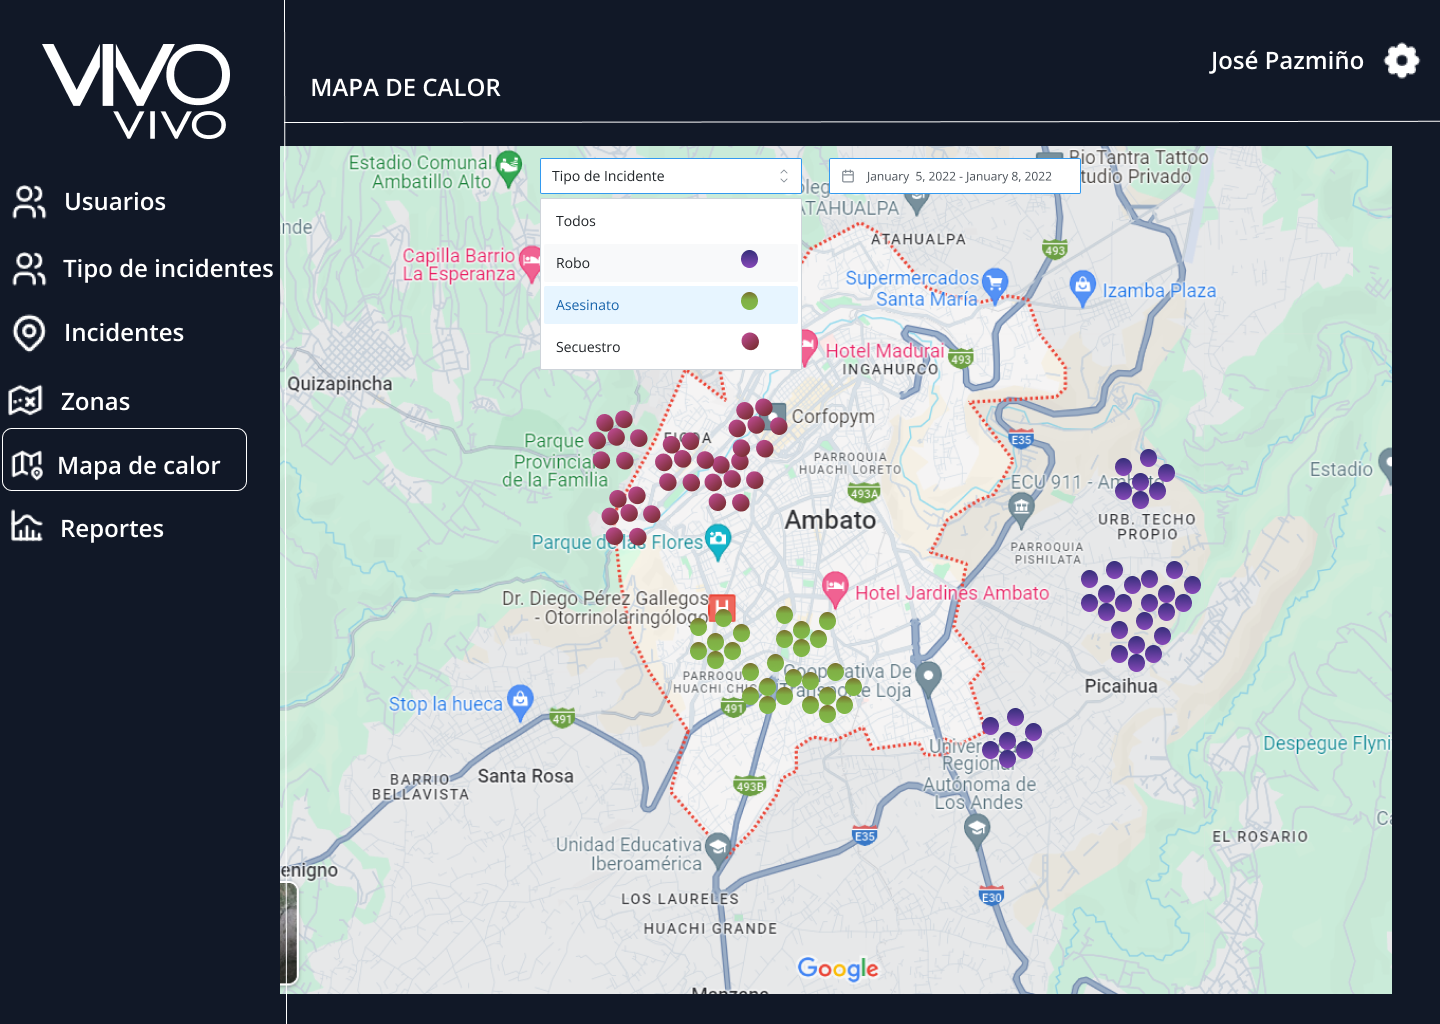
\includegraphics[width=0.6\textwidth]{chapters/III-resultados-y-discusion/resources/images/prototipo-mapa-de-calor-web.png}
%     \caption{Prototipo de la interfaz para visualizar el mapa de calor}
%     \label{fig:prototipo-interfaz-usuario-web-9}
% \end{figure}


\begin{longtable}{|p{6.7cm}|p{6.7cm}|}
    \caption{Historia de usuario 9: Iniciar sesión aplicación móvil} \label{tab:historia-9}
    \\
    \hline
    \multicolumn{2}{|c|}{\textbf{Historia de Usuario}}                                                                                               \\
    \hline

    \endfirsthead

    \hline
    \endhead

    \hline
    \multicolumn{2}{|c|}{{Continua en la siguiente página}}                                                                                          \\
    \hline
    \endfoot

    \hline
    \endlastfoot

    \textbf{Número:} 9                                  & \textbf{Usuario:} Ciudadano                                                                \\
    \hline
    \multicolumn{2}{|l|}{\textbf{Nombre de la historia:} Iniciar sesión sistema móvil}                                                               \\
    \hline
    \textbf{Prioridad en negocio}  Alta                 & \textbf{Riesgo en desarrollo:} Medio                                                       \\
    \hline
    \textbf{\textbf{Puntos estimados:}en desarrollo:} 8 & \textbf{Iteración asignada:} 3                                                             \\
    \hline
    \multicolumn{2}{|l|}{\textbf{Programador responsable:} José Pazmiño }                                                                            \\
    \hline
    \multicolumn{2}{|p{13.4cm}|}{\textbf{Descripción:} Como ciudadano, quiero iniciar sesión en el sistema móvil para acceder a sus funcionalidades} \\
    \hline
    \multicolumn{2}{|c|}{\textbf{Criterios de aceptación}}                                                                                           \\
    \hline
    \multicolumn{2}{|p{13.4cm}|}{
    \begin{itemize}[label={},leftmargin=*, nosep]
        \item \textbf{Criterio 1:} Dado que el ciudadano ingrese su correo y contraseña de forma correcta cuando presione el botón de inicio de sesión, la aplicación deberá redirigirlo a la pantalla principal de la aplicación.
        \item \textbf{Criterio 2:} Dado que el ciudadano ingrese su correo y contraseña de forma incorrecta cuando presione el botón de inicio de sesión, la aplicación deberá mostrar un mensaje de error.
    \end{itemize}
    }                                                                                                                                                \\
\end{longtable}


% \begin{figure}[H]
%     \centering
%     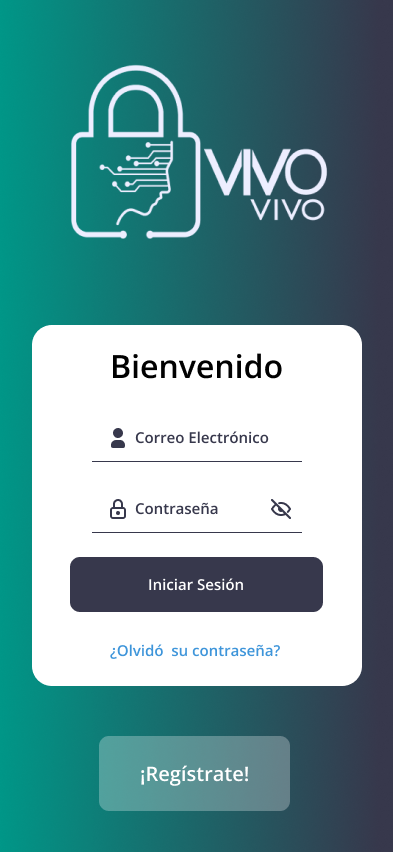
\includegraphics[width=0.4\textwidth]{chapters/III-resultados-y-discusion/resources/images/prototipo-inicio-sesion-mobile.png}
%     \caption{Prototipo de la interfaz para iniciar sesión en la aplicación móvil}
%     \label{fig:prototipo-interfaz-usuario-web-10}
% \end{figure}


\begin{longtable}{|p{6.7cm}|p{6.7cm}|}
    \caption{Historia de usuario 10: Cerrar sesión aplicación móvil} \label{tab:historia-10}
    \\
    \hline
    \multicolumn{2}{|c|}{\textbf{Historia de Usuario}}                                                                                                  \\
    \hline

    \endfirsthead

    \hline
    \endhead

    \hline
    \multicolumn{2}{|c|}{{Continua en la siguiente página}}                                                                                             \\
    \hline
    \endfoot

    \hline
    \endlastfoot

    \textbf{Número:} 10                                 & \textbf{Usuario:} Ciudadano                                                                   \\
    \hline
    \multicolumn{2}{|l|}{\textbf{Nombre de la historia:} Cerrar sesión aplicación móvil}                                                                \\
    \hline
    \textbf{Prioridad en negocio}  Alta                 & \textbf{Riesgo en desarrollo:} Medio                                                          \\
    \hline
    \textbf{\textbf{Puntos estimados:}en desarrollo:} 4 & \textbf{Iteración asignada:} 3                                                                \\
    \hline
    \multicolumn{2}{|l|}{\textbf{Programador responsable:} José Pazmiño }                                                                               \\
    \hline
    \multicolumn{2}{|p{13.4cm}|}{\textbf{Descripción:} Como ciudadano, quiero cerrar sesión en la aplicación móvil para finalizar mi sesión de trabajo} \\
    \hline
    \multicolumn{2}{|c|}{\textbf{Criterios de aceptación}}                                                                                              \\
    \hline
    \multicolumn{2}{|p{13.4cm}|}{
    \begin{itemize}[label={},leftmargin=*, nosep]
        \item \textbf{Criterio 1:} Dado que el ciudadano presione el botón de cerrar sesión desde cualquier pantalla, la aplicación deberá redirigirlo a la pantalla de inicio de sesión.
    \end{itemize}
    }                                                                                                                                                   \\
\end{longtable}


% \begin{figure}[H]
%     \centering
%     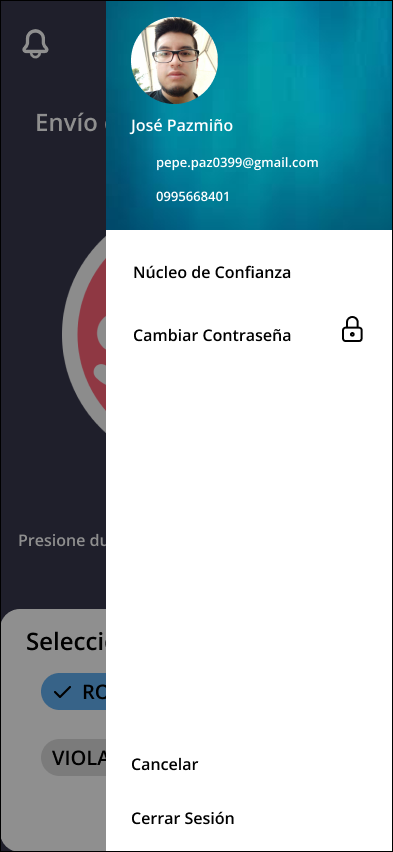
\includegraphics[width=0.4\textwidth]{chapters/III-resultados-y-discusion/resources/images/prototipo-menu-mobile.png}
%     \caption{Prototipo de la interfaz para cerrar sesión en la aplicación móvil}
%     \label{fig:prototipo-interfaz-usuario-web-11}
% \end{figure}



\begin{longtable}{|p{6.7cm}|p{6.7cm}|}
    \caption{Historia de usuario 11: Registro de usuario} \label{tab:historia-11}
    \\
    \hline
    \multicolumn{2}{|c|}{\textbf{Historia de Usuario}}                                                                                \\
    \hline

    \endfirsthead

    \hline
    \endhead

    \hline
    \multicolumn{2}{|c|}{{Continua en la siguiente página}}                                                                           \\
    \hline
    \endfoot

    \hline
    \endlastfoot

    \textbf{Número:} 11                                  & \textbf{Usuario:} Ciudadano                                                \\
    \hline
    \multicolumn{2}{|l|}{\textbf{Nombre de la historia:} Registro de usuario}                                                         \\
    \hline
    \textbf{Prioridad en negocio}  Alta                  & \textbf{Riesgo en desarrollo:} Medio                                       \\
    \hline
    \textbf{\textbf{Puntos estimados:}en desarrollo:} 11 & \textbf{Iteración asignada:} 3                                             \\
    \hline
    \multicolumn{2}{|l|}{\textbf{Programador responsable:} José Pazmiño }                                                             \\
    \hline
    \multicolumn{2}{|p{13.4cm}|}{\textbf{Descripción:} Como ciudadano, quiero ingresar mis datos y fotografía mediante un formulario} \\
    \hline
    \multicolumn{2}{|c|}{\textbf{Criterios de aceptación}}                                                                            \\
    \hline
    \multicolumn{2}{|p{13.4cm}|}{
    \begin{itemize}[label={},leftmargin=*, nosep]
        \item \textbf{Criterio 1:} El ciudadano debe poder ingresar sus datos personales y fotografía mediante un formulario.
    \end{itemize}
    }                                                                                                                                 \\
\end{longtable}


% \begin{figure}[H]
%     \centering
%     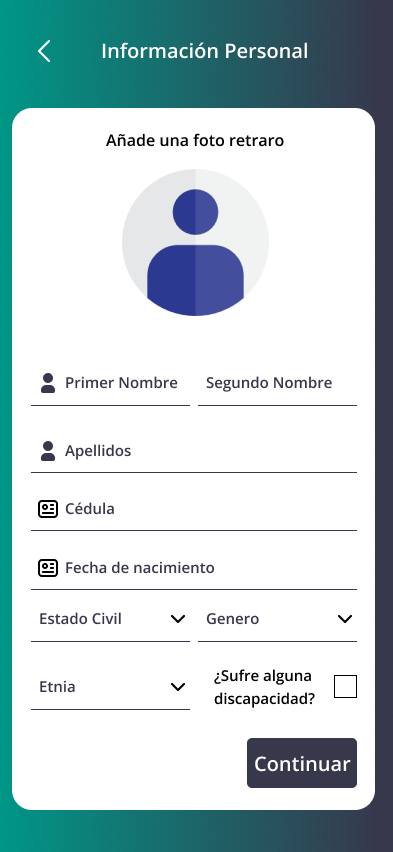
\includegraphics[width=0.4\textwidth]{chapters/III-resultados-y-discusion/resources/images/prototipo-registro-mobile.png}
%     \caption{Prototipo de la interfaz para el registro de usuarios en la aplicación móvil}
%     \label{fig:prototipo-interfaz-usuario-web-12}
% \end{figure}


\begin{longtable}{|p{6.7cm}|p{6.7cm}|}
    \caption{Historia de usuario 12: Asignar miembros al grupo familiar} \label{tab:historia-12}
    \\
    \hline
    \multicolumn{2}{|c|}{\textbf{Historia de Usuario}}                                                                                               \\
    \hline

    \endfirsthead

    \hline
    \endhead

    \hline
    \multicolumn{2}{|c|}{{Continua en la siguiente página}}                                                                                          \\
    \hline
    \endfoot

    \hline
    \endlastfoot

    \textbf{Número:} 12                                  & \textbf{Usuario:} Ciudadano                                                               \\
    \hline
    \multicolumn{2}{|l|}{\textbf{Nombre de la historia:} Asignar miembros al grupo familiar}                                                         \\
    \hline
    \textbf{Prioridad en negocio}  Alta                  & \textbf{Riesgo en desarrollo:} Medio                                                      \\
    \hline
    \textbf{\textbf{Puntos estimados:}en desarrollo:} 18 & \textbf{Iteración asignada:} 4                                                            \\
    \hline
    \multicolumn{2}{|l|}{\textbf{Programador responsable:} José Pazmiño }                                                                            \\
    \hline
    \multicolumn{2}{|p{13.4cm}|}{\textbf{Descripción:} Como ciudadano, quiero asignar miembros al grupo familiar para recibir alertas de emergencia} \\
    \hline
    \multicolumn{2}{|c|}{\textbf{Criterios de aceptación}}                                                                                           \\
    \hline
    \multicolumn{2}{|p{13.4cm}|}{
    \begin{itemize}[label={},leftmargin=*, nosep]
        \item \textbf{Criterio 1:} El ciudadano debe poder asignar miembros al grupo familiar para recibir alertas de emergencia.
        \item \textbf{Criterio 2:} El ciudadano debe poder visualizar los miembros asignados al grupo familiar.
              % \item \textbf{Criterio 3:} El ciudadano debe poder desasignar miembros del grupo familiar.
    \end{itemize}
    }                                                                                                                                                \\
\end{longtable}


% \begin{figure}[H]
%     \centering
%     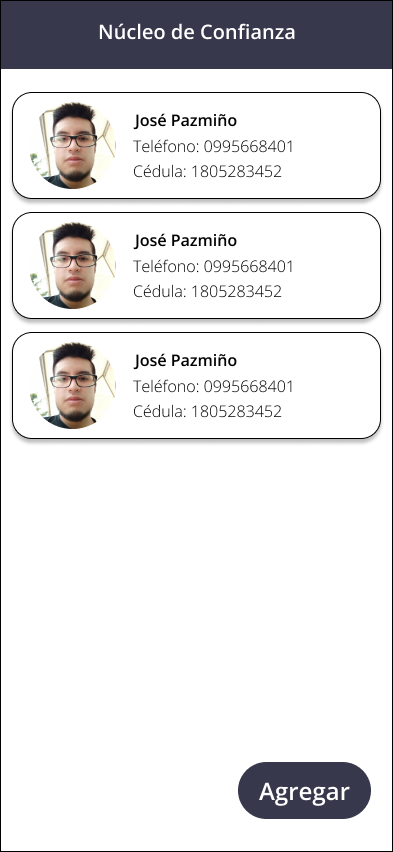
\includegraphics[width=0.4\textwidth]{chapters/III-resultados-y-discusion/resources/images/prototipo-grupo-familiar-mobile.png}
%     \caption{Prototipo de la interfaz para visualizar los miembros del grupo familiar}
%     \label{fig:prototipo-interfaz-usuario-web-13}
% \end{figure}

% \begin{figure}[H]
%     \centering
%     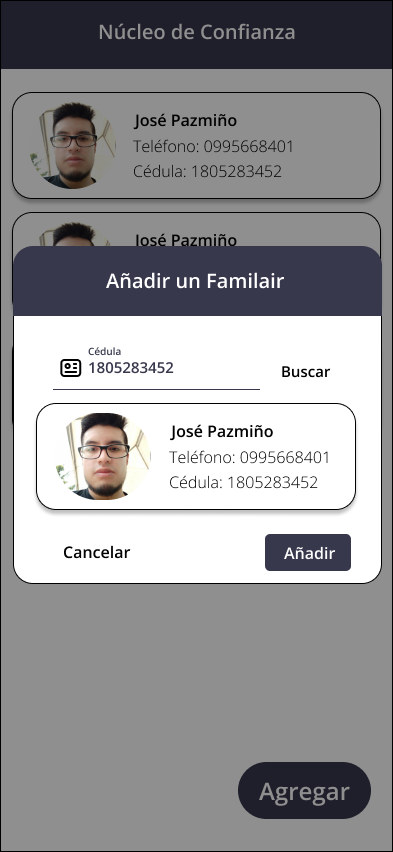
\includegraphics[width=0.4\textwidth]{chapters/III-resultados-y-discusion/resources/images/prototipo-agregar-miembro-mobile.png}
%     \caption{Prototipo de la interfaz para agregar miembros al grupo familiar}
%     \label{fig:prototipo-interfaz-usuario-web-14}
% \end{figure}


\begin{longtable}{|p{6.7cm}|p{6.7cm}|}
    \caption{Historia de usuario 13: Enviar alerta de incidente} \label{tab:historia-13}
    \\
    \hline
    \multicolumn{2}{|c|}{\textbf{Historia de Usuario}}                                                                                                                      \\
    \hline

    \endfirsthead

    \hline
    \endhead

    \hline
    \multicolumn{2}{|c|}{{Continua en la siguiente página}}                                                                                                                 \\
    \hline
    \endfoot

    \hline
    \endlastfoot

    \textbf{Número:} 13                                  & \textbf{Usuario:} Ciudadano                                                                                      \\
    \hline
    \multicolumn{2}{|l|}{\textbf{Nombre de la historia:} Enviar alerta de incidente}                                                                                        \\
    \hline
    \textbf{Prioridad en negocio}  Alta                  & \textbf{Riesgo en desarrollo:} Medio                                                                             \\
    \hline
    \textbf{\textbf{Puntos estimados:}en desarrollo:} 21 & \textbf{Iteración asignada:} 4                                                                                   \\
    \hline
    \multicolumn{2}{|l|}{\textbf{Programador responsable:} José Pazmiño }                                                                                                   \\
    \hline
    \multicolumn{2}{|p{13.4cm}|}{\textbf{Descripción:} Como ciudadano, quiero enviar una alerta de incidente para notificar a las autoridades sobre un incidente delictivo} \\
    \hline
    \multicolumn{2}{|c|}{\textbf{Criterios de aceptación}}                                                                                                                  \\
    \hline
    \multicolumn{2}{|p{13.4cm}|}{
    \begin{itemize}[label={},leftmargin=*, nosep]
        \item \textbf{Criterio 1:} El ciudadano debe poder enviar una alerta de incidente para notificar a sus familiares y entes de control sobre una emergencia.
    \end{itemize}
    }                                                                                                                                                                       \\
\end{longtable}


% \begin{figure}[H]
%     \centering
%     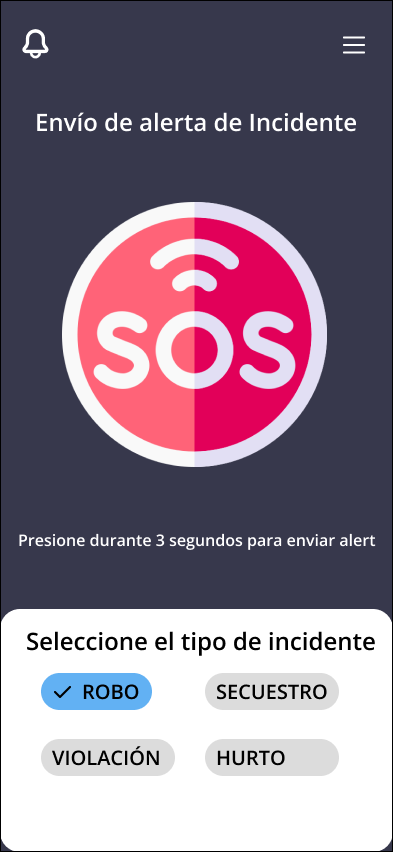
\includegraphics[width=0.4\textwidth]{chapters/III-resultados-y-discusion/resources/images/prototipo-inicio-mobile.png}
%     \caption{Prototipo de la interfaz para enviar una alerta de incidente}
%     \label{fig:prototipo-interfaz-usuario-web-16}
% \end{figure}

% \begin{figure}[H]
%     \centering
%     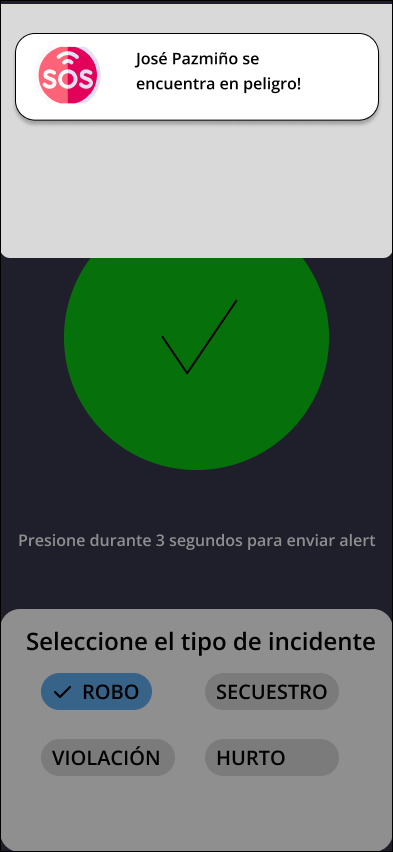
\includegraphics[width=0.4\textwidth]{chapters/III-resultados-y-discusion/resources/images/prototipo-notificacion-alerta.png}
%     \caption{Prototipo de la interfaz para visualizar la notificación de alerta de incidente}
%     \label{fig:prototipo-interfaz-usuario-web-17}
% \end{figure}


\begin{longtable}{|p{6.7cm}|p{6.7cm}|}
    \caption{Historia de usuario 14: Visualizar alertas de emergencia de familiares} \label{tab:historia-14}
    \\
    \hline
    \multicolumn{2}{|c|}{\textbf{Historia de Usuario}}                                                                                                                                               \\
    \hline

    \endfirsthead

    \hline
    \endhead

    \hline
    \multicolumn{2}{|c|}{{Continua en la siguiente página}}                                                                                                                                          \\
    \hline
    \endfoot

    \hline
    \endlastfoot

    \textbf{Número:} 14                                  & \textbf{Usuario:} Ciudadano                                                                                                               \\
    \hline
    \multicolumn{2}{|l|}{\textbf{Nombre de la historia:} Visualizar alertas de emergencia de familiares}                                                                                             \\
    \hline
    \textbf{Prioridad en negocio}  Alta                  & \textbf{Riesgo en desarrollo:} Medio                                                                                                      \\
    \hline
    \textbf{\textbf{Puntos estimados:}en desarrollo:} 21 & \textbf{Iteración asignada:} 4                                                                                                            \\
    \hline
    \multicolumn{2}{|l|}{\textbf{Programador responsable:} José Pazmiño }                                                                                                                            \\
    \hline
    \multicolumn{2}{|p{13.4cm}|}{\textbf{Descripción:} Como ciudadano, quiero visualizar mediante un mapa las alertas de emergencia enviadas por mis familiares así como su posición en tiempo real} \\
    \hline
    \multicolumn{2}{|c|}{\textbf{Criterios de aceptación}}                                                                                                                                           \\
    \hline
    \multicolumn{2}{|p{13.4cm}|}{
    \begin{itemize}[label={},leftmargin=*, nosep]
        \item \textbf{Criterio 1:} El ciudadano debe poder visualizar mediante un mapa las alertas de emergencia enviadas por los miembros de su grupo familiar así como su posición en tiempo real.
    \end{itemize}
    }                                                                                                                                                                                                \\
\end{longtable}


% \begin{figure}[H]
%     \centering
%     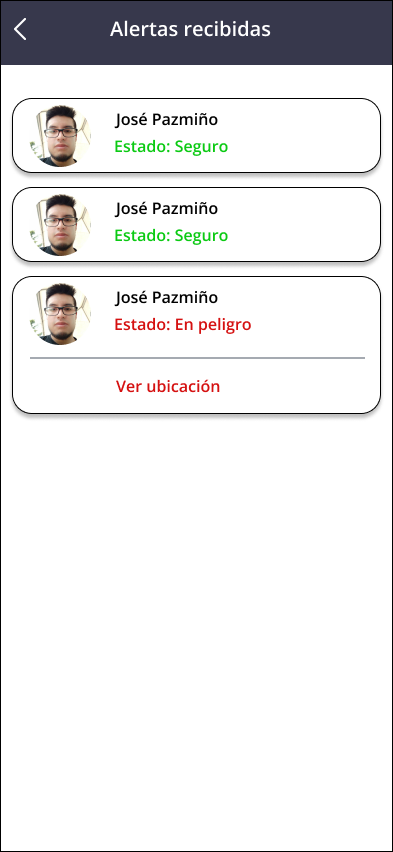
\includegraphics[width=0.4\textwidth]{chapters/III-resultados-y-discusion/resources/images/prototipo-alertas-mobile.png}
%     \caption{Prototipo de la interfaz para visualizar las alertas de emergencia de familiares}
%     \label{fig:prototipo-interfaz-usuario-web-18}
% \end{figure}

% \begin{figure}[H]
%     \centering
%     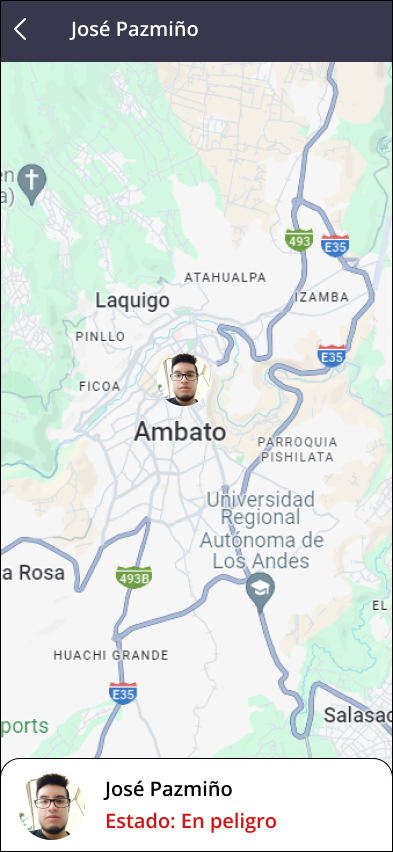
\includegraphics[width=0.4\textwidth]{chapters/III-resultados-y-discusion/resources/images/prototipo-ubicacion-alerta-mobile.png}
%     \caption{Prototipo de la interfaz para visualizar la ubicación de la alerta de emergencia de un familiar}
%     \label{fig:prototipo-interfaz-usuario-web-19}
% \end{figure}


\begin{longtable}{|p{6.7cm}|p{6.7cm}|}
    \caption{Historia de usuario 15: Visualizar alertas de emergencia de ciudadanos} \label{tab:historia-15}
    \\
    \hline
    \multicolumn{2}{|c|}{\textbf{Historia de Usuario}}                                                                                                                                                                    \\
    \hline

    \endfirsthead

    \hline
    \endhead

    \hline
    \multicolumn{2}{|c|}{{Continua en la siguiente página}}                                                                                                                                                               \\
    \hline
    \endfoot

    \hline
    \endlastfoot

    \textbf{Número:} 15                                  & \textbf{Usuario:} Policía                                                                                                                                      \\
    \hline
    \multicolumn{2}{|l|}{\textbf{Nombre de la historia:} Visualizar alertas de emergencia de ciudadanos}                                                                                                                  \\
    \hline
    \textbf{Prioridad en negocio}  Alta                  & \textbf{Riesgo en desarrollo:} Medio                                                                                                                           \\
    \hline
    \textbf{\textbf{Puntos estimados:}en desarrollo:} 11 & \textbf{Iteración asignada:} 4                                                                                                                                 \\
    \hline
    \multicolumn{2}{|l|}{\textbf{Programador responsable:} José Pazmiño }                                                                                                                                                 \\
    \hline
    \multicolumn{2}{|p{13.4cm}|}{\textbf{Descripción:} Como policía, quiero visualizar mediante un mapa las alertas de emergencia enviadas por los ciudadanos así como su posición en tiempo real y el tipo de incidente} \\
    \hline
    \multicolumn{2}{|c|}{\textbf{Criterios de aceptación}}                                                                                                                                                                \\
    \hline
    \multicolumn{2}{|p{13.4cm}|}{
    \begin{itemize}[label={},leftmargin=*, nosep]
        \item \textbf{Criterio 1:} El policía debe poder visualizar mediante un mapa las alertas de emergencia enviadas por los ciudadanos así como su posición en tiempo real y el tipo de incidente.
    \end{itemize}
    }
    \\
\end{longtable}


% \begin{figure}[H]
%     \centering
%     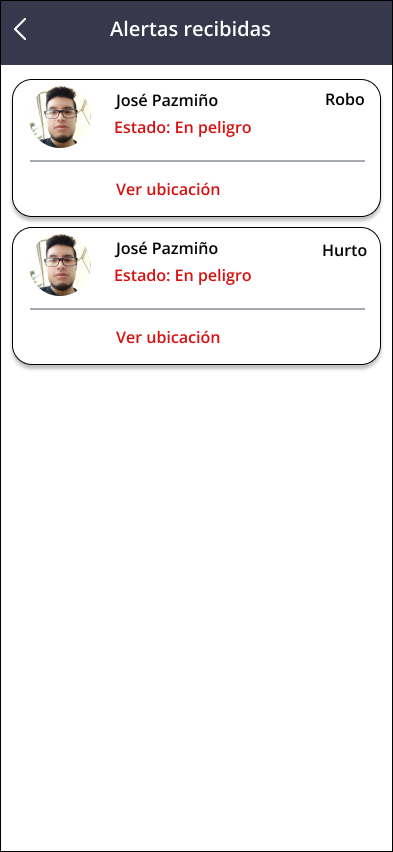
\includegraphics[width=0.4\textwidth]{chapters/III-resultados-y-discusion/resources/images/prototipo-alertas-policia.png}
%     \caption{Prototipo de la interfaz para visualizar las alertas de emergencia de ciudadanos}
%     \label{fig:prototipo-interfaz-usuario-web-20}
% \end{figure}

% \begin{figure}[H]
%     \centering
%     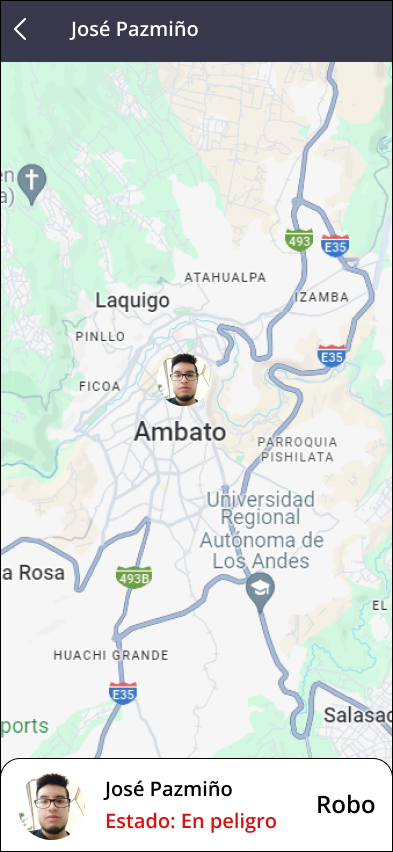
\includegraphics[width=0.4\textwidth]{chapters/III-resultados-y-discusion/resources/images/prototipo-ubicacion-alerta-policia.png}
%     \caption{Prototipo de la interfaz para visualizar la ubicación de la alerta de emergencia de un ciudadano}
%     \label{fig:prototipo-interfaz-usuario-web-21}
% \end{figure}


\begin{longtable}{|p{6.7cm}|p{6.7cm}|}
    \caption{Historia de usuario 16: Cambiar contraseña} \label{tab:historia-16}
    \\
    \hline
    \multicolumn{2}{|c|}{\textbf{Historia de Usuario}}                                                                                      \\
    \hline

    \endfirsthead

    \hline
    \endhead

    \hline
    \multicolumn{2}{|c|}{{Continua en la siguiente página}}                                                                                 \\
    \hline
    \endfoot

    \hline
    \endlastfoot

    \textbf{Número:} 16                                  & \textbf{Usuario:} Ciudadano                                                      \\
    \hline
    \multicolumn{2}{|l|}{\textbf{Nombre de la historia:} Cambiar contraseña}                                                                \\
    \hline
    \textbf{Prioridad en negocio}  Media                 & \textbf{Riesgo en desarrollo:} Medio                                             \\
    \hline
    \textbf{\textbf{Puntos estimados:}en desarrollo:} 14 & \textbf{Iteración asignada:} 5                                                   \\
    \hline
    \multicolumn{2}{|l|}{\textbf{Programador responsable:} José Pazmiño }                                                                   \\
    \hline
    \multicolumn{2}{|p{13.4cm}|}{\textbf{Descripción:} Como ciudadano, quiero cambiar mi contraseña para mejorar la seguridad de mi cuenta} \\
    \hline
    \multicolumn{2}{|c|}{\textbf{Criterios de aceptación}}                                                                                  \\
    \hline
    \multicolumn{2}{|p{13.4cm}|}{
    \begin{itemize}[label={},leftmargin=*, nosep]
        \item \textbf{Criterio 1:} El ciudadano debe poder cambiar su contraseña para mejorar la seguridad de su cuenta.
    \end{itemize}
    }
    \\
\end{longtable}


% \begin{figure}[H]
%     \centering
%     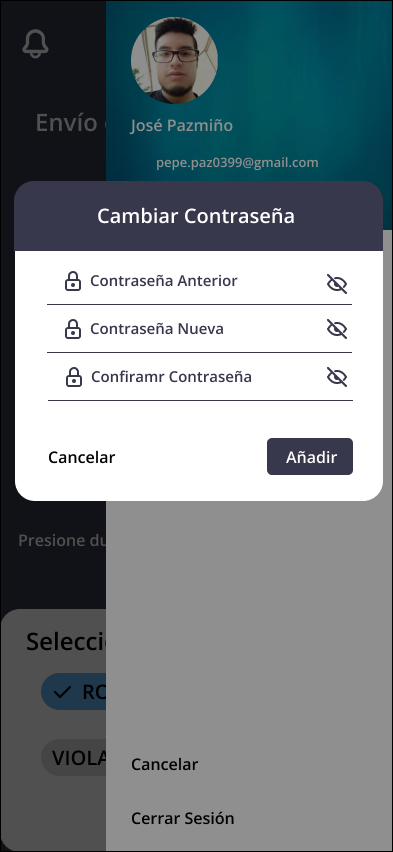
\includegraphics[width=0.4\textwidth]{chapters/III-resultados-y-discusion/resources/images/prototipo-cambiar-contrasena-mobile.png}
%     \caption{Prototipo de la interfaz para cambiar la contraseña en la aplicación móvil}
%     \label{fig:prototipo-interfaz-usuario-web-22}
% \end{figure}


\begin{longtable}{|p{6.7cm}|p{6.7cm}|}
    \caption{Historia de usuario 17: Recuperar contraseña} \label{tab:historia-17}
    \\
    \hline
    \multicolumn{2}{|c|}{\textbf{Historia de Usuario}}                                                                      \\
    \hline

    \endfirsthead

    \hline
    \endhead

    \hline
    \multicolumn{2}{|c|}{{Continua en la siguiente página}}                                                                 \\
    \hline
    \endfoot

    \hline
    \endlastfoot

    \textbf{Número:} 17                                  & \textbf{Usuario:} Ciudadano                                      \\
    \hline
    \multicolumn{2}{|l|}{\textbf{Nombre de la historia:} Recuperar contraseña}                                              \\
    \hline
    \textbf{Prioridad en negocio}  Media                 & \textbf{Riesgo en desarrollo:} Medio                             \\
    \hline
    \textbf{\textbf{Puntos estimados:}en desarrollo:} 15 & \textbf{Iteración asignada:} 5                                   \\
    \hline
    \multicolumn{2}{|l|}{\textbf{Programador responsable:} José Pazmiño }                                                   \\
    \hline
    \multicolumn{2}{|p{13.4cm}|}{\textbf{Descripción:} Como ciudadano, quiero recuperar mi contraseña en caso de olvidarla} \\
    \hline
    \multicolumn{2}{|c|}{\textbf{Criterios de aceptación}}                                                                  \\
    \hline
    \multicolumn{2}{|p{13.4cm}|}{
    \begin{itemize}[label={},leftmargin=*, nosep]
        \item \textbf{Criterio 1:} El ciudadano debe poder recuperar su contraseña en caso de olvidarla.
    \end{itemize}
    }
    \\
\end{longtable}


% \begin{figure}[H]
%     \centering
%     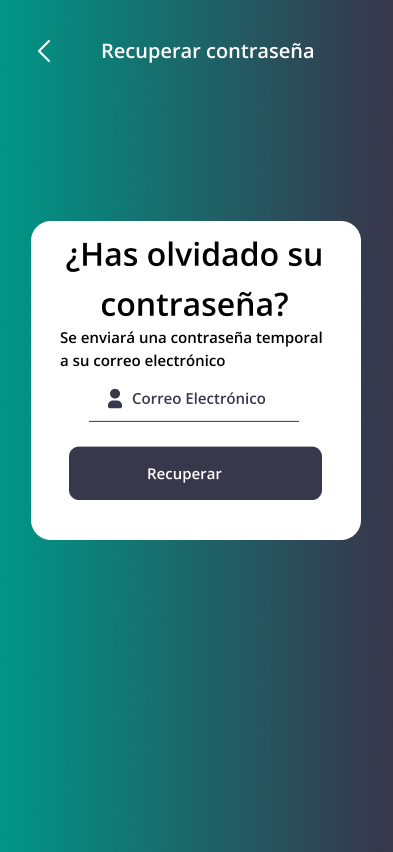
\includegraphics[width=0.4\textwidth]{chapters/III-resultados-y-discusion/resources/images/prototipo-recuperar-contrasena-mobile.png}
%     \caption{Prototipo de la interfaz para recuperar la contraseña en la aplicación móvil}
%     \label{fig:prototipo-interfaz-usuario-web-23}
% \end{figure}


\begin{longtable}{|p{6.7cm}|p{6.7cm}|}
    \caption{Historia de usuario 18: Desarrollar modelo analítico de BI} \label{tab:historia-18}
    \\
    \hline
    \multicolumn{2}{|c|}{\textbf{Historia de Usuario}}                                                                                           \\
    \hline

    \endfirsthead

    \hline
    \endhead

    \hline
    \multicolumn{2}{|c|}{{Continua en la siguiente página}}                                                                                      \\
    \hline
    \endfoot

    \hline
    \endlastfoot

    \textbf{Número:} 18                                  & \textbf{Usuario:} Administrador                                                       \\
    \hline
    \multicolumn{2}{|l|}{\textbf{Nombre de la historia:} Desarrollar modelo analítico de BI}                                                     \\
    \hline
    \textbf{Prioridad en negocio}  Alta                  & \textbf{Riesgo en desarrollo:} Medio                                                  \\
    \hline
    \textbf{\textbf{Puntos estimados:}en desarrollo:} 41 & \textbf{Iteración asignada:} 5                                                        \\
    \hline
    \multicolumn{2}{|l|}{\textbf{Programador responsable:} José Pazmiño }                                                                        \\
    \hline
    \multicolumn{2}{|p{13.4cm}|}{\textbf{Descripción:} Como administrador, quiero visualizar informes detallados sobre los incidentes ocurridos} \\
    \hline
    \multicolumn{2}{|c|}{\textbf{Criterios de aceptación}}                                                                                       \\
    \hline
    \multicolumn{2}{|p{13.4cm}|}{
    \begin{itemize}[label={},leftmargin=*, nosep]
        \item \textbf{Criterio 1:} El administrador debe poder visualizar informes detallados sobre los incidentes ocurridos.
        \item  \textbf{Criterio 2:} El administrador debe poder la información al realizar al  click en las gráficas.
    \end{itemize}
    }
    \\
\end{longtable}